% Figure and table floats, defined as macros so that each can be placed in the text where it is first cited
% (\placefloat{<label>}). Main figures float near their text ([tbp]); supplementary floats are placed in
% Additional file 1 (sections/additional_file1.tex), each on its own page.
\makeatletter
\newcommand{\placefloat}[1]{\@ifundefined{float@#1}{\PackageError{figure_defs}{No float #1}{}}{\@nameuse{float@#1}}}
\makeatother

% fig:1
\expandafter\long\expandafter\def\csname float@fig:1\endcsname{%
\begin{figure}[tbp]
\centering
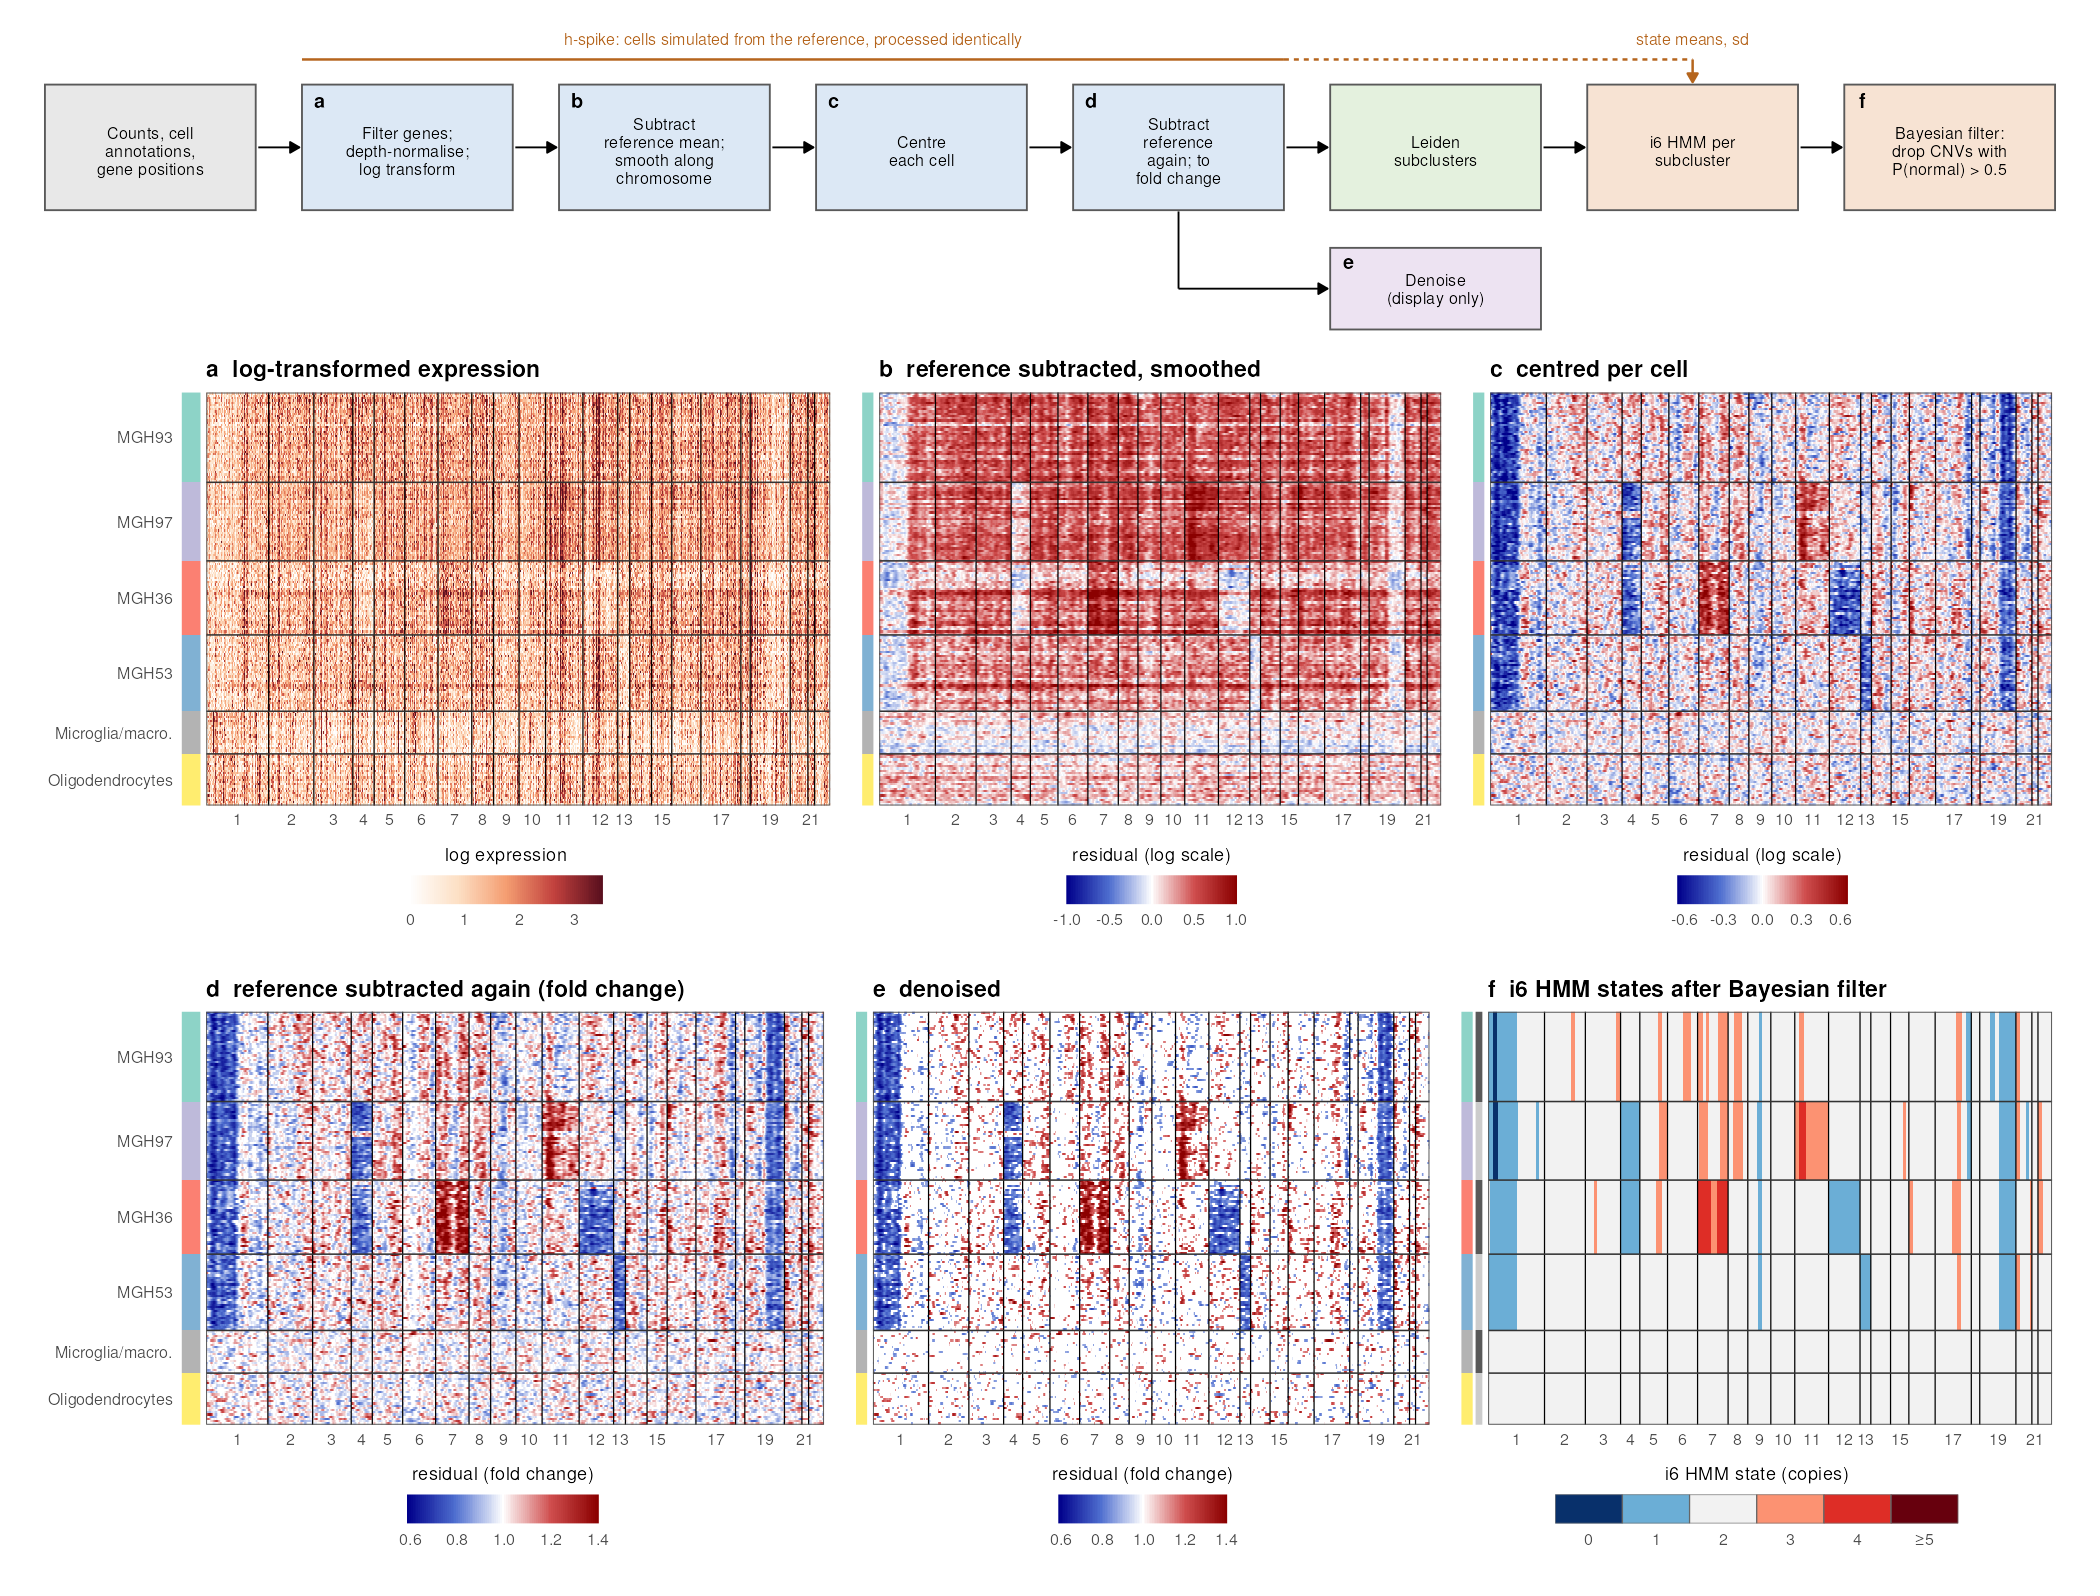
\includegraphics[width=\textwidth]{figures/fig1_workflow.png}
\caption{\textbf{The inferCNV workflow.} Top, schematic of the main steps; letters mark the steps shown below. Heatmaps, snapshots from the 184-cell oligodendroglioma example data set (142 malignant cells from four tumours above, 42 reference cells below; columns are genes ordered by genomic position, chromosome numbers below). (a) Log-transformed expression after gene filtering and depth normalisation. (b) Residual expression after subtraction of the reference mean and smoothing along each chromosome (log scale). (c) After per-cell centering. (d) After the second reference subtraction, shown on the fold-change scale. (e) After denoising (\texttt{denoise\ =\ TRUE}; same colour scale as d). (f) i6 HMM states after Bayesian filtering (\texttt{BayesMaxPNormal\ =\ 0.5}); the HMM is run per Leiden subcluster (grey bar; one subcluster per tumour in this data set) on the residuals in (d), and each cell is shown with the states of its subcluster. Panels (e) and (f) are alternative outputs derived from (d). The h-spike (top, orange) is processed alongside the data and supplies the HMM emission parameters (Fig.~\ref{fig:2}).}
\label{fig:1}
\end{figure}}

% fig:2
\expandafter\long\expandafter\def\csname float@fig:2\endcsname{%
\begin{figure}[tbp]
\centering
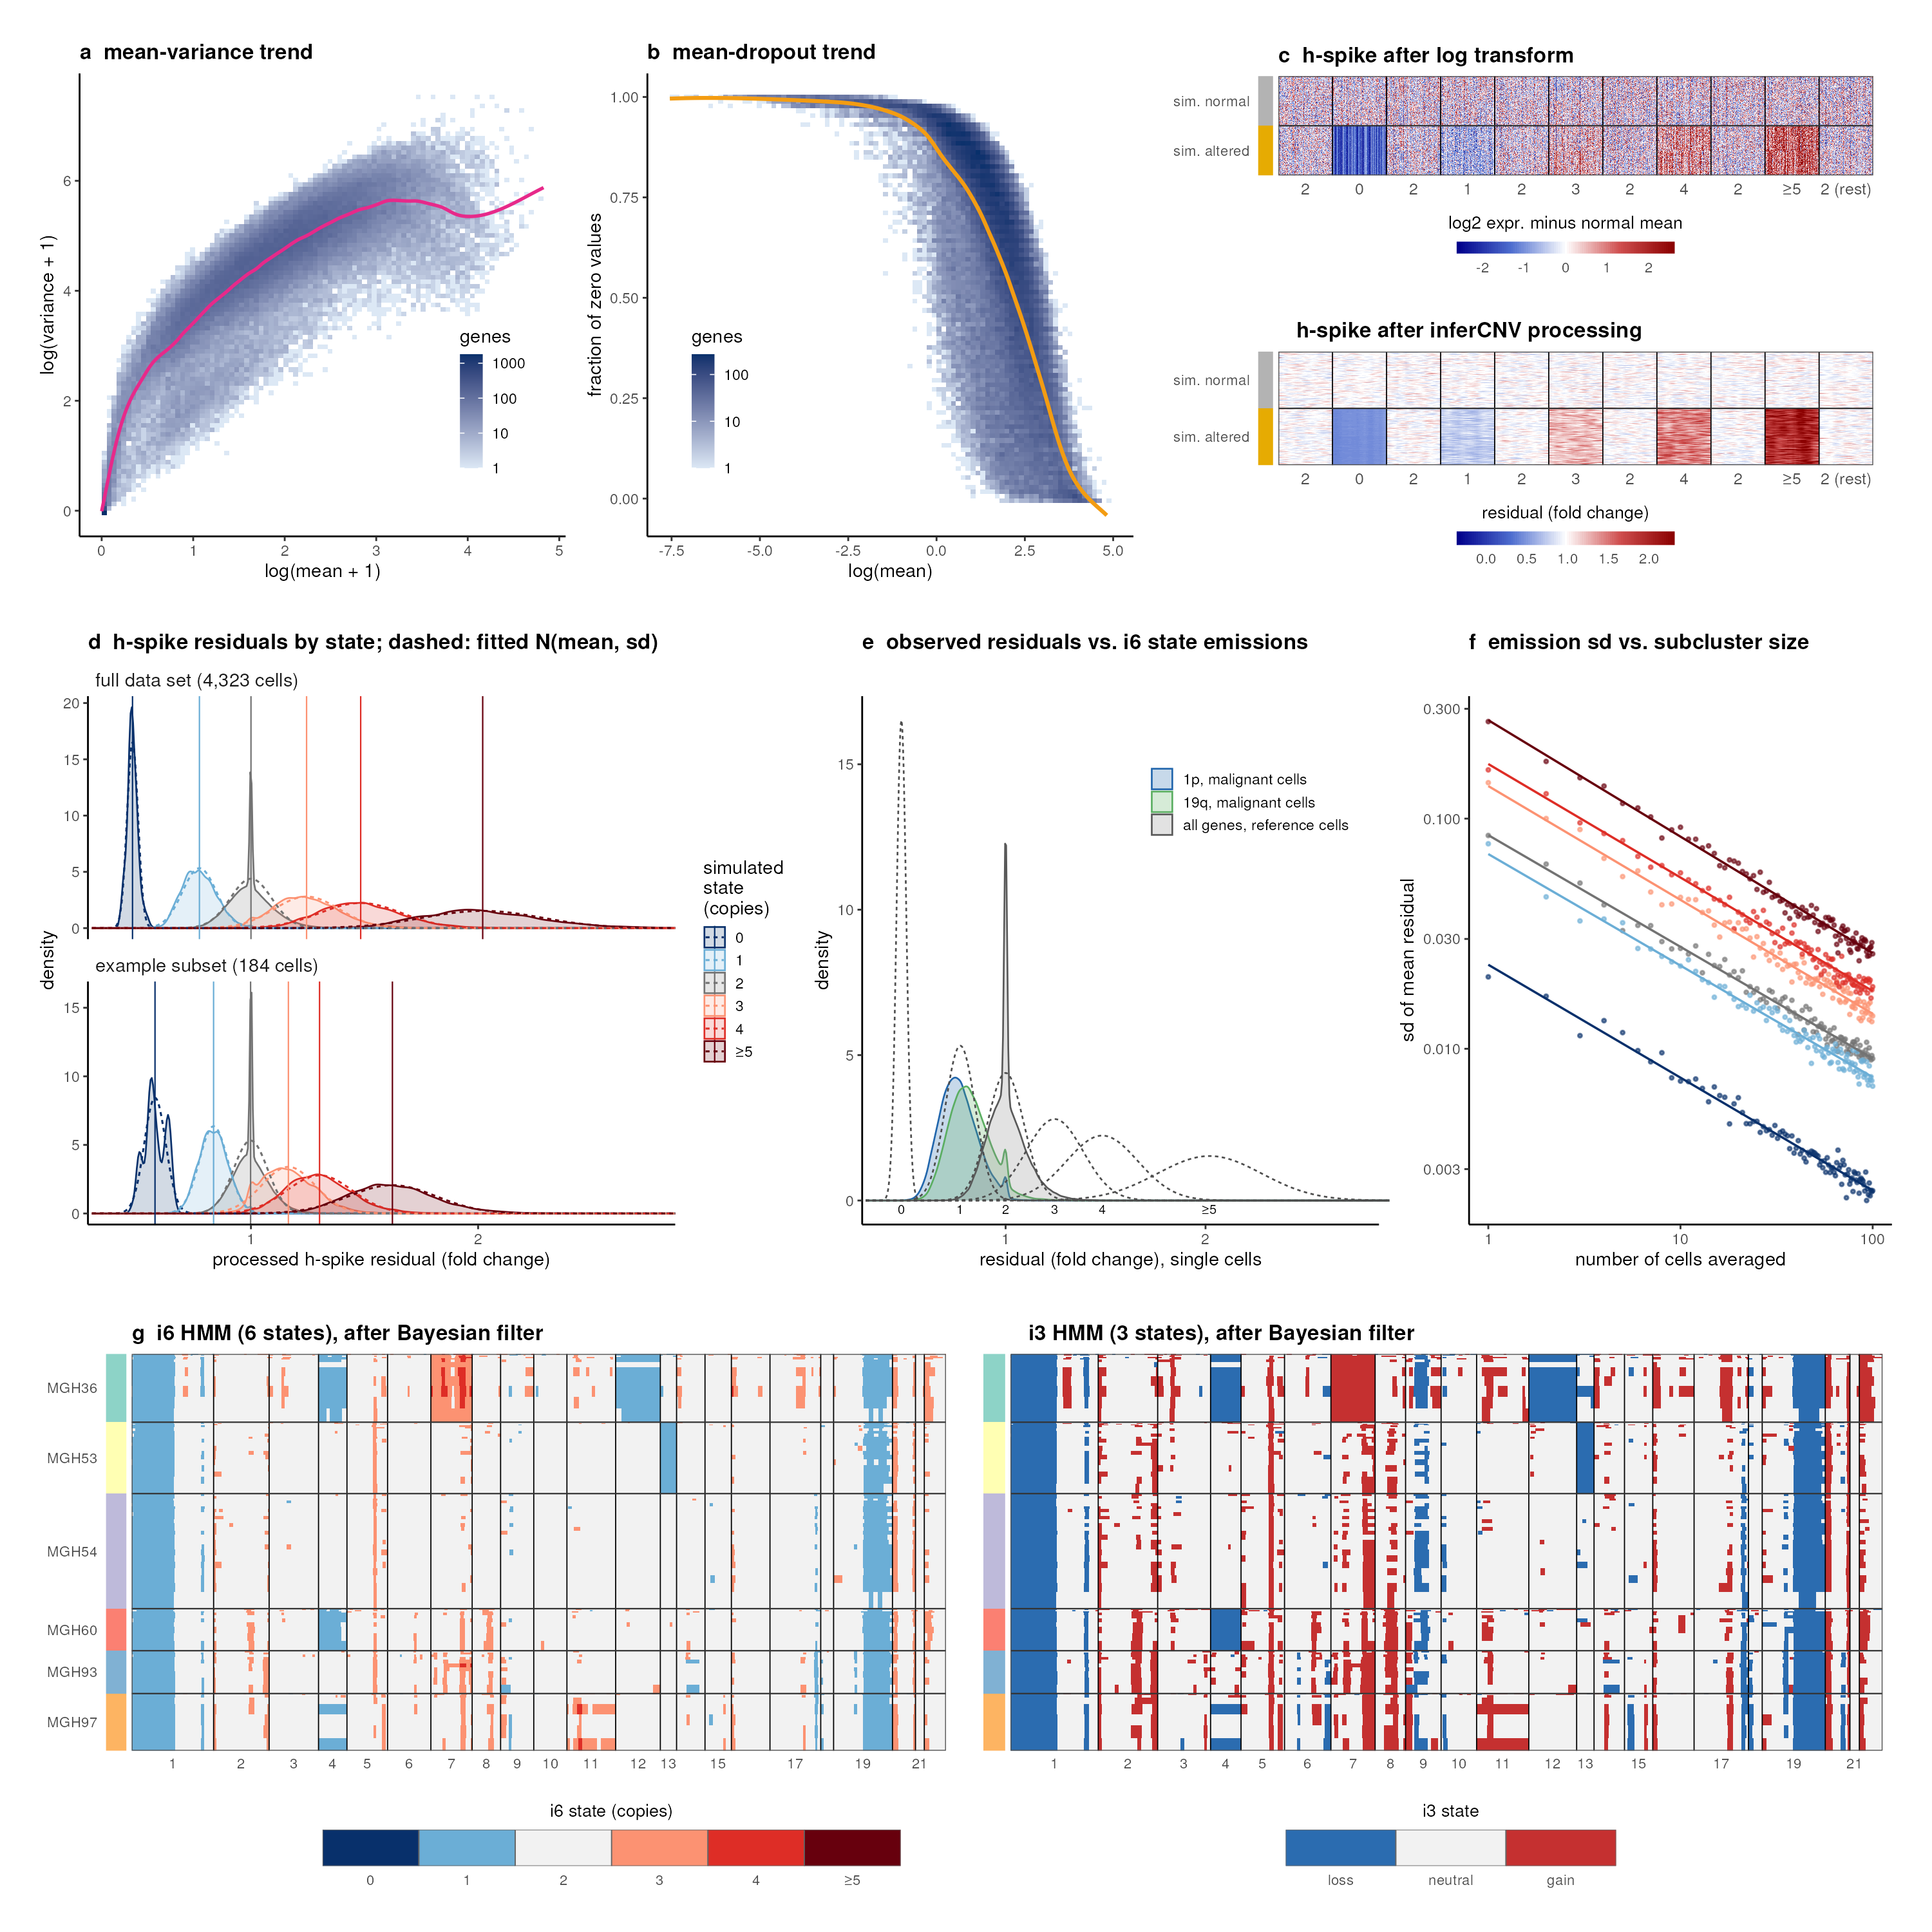
\includegraphics[width=\textwidth]{figures/fig2_hspike.png}
\caption{\textbf{In-silico spike-in (h-spike) calibration of the HMM.} Full oligodendroglioma data set (4,043 malignant and 280 reference cells), with the 184-cell example for comparison in (d). (a) Mean--variance and (b) mean--dropout relationships of the depth-normalised data, computed per annotation group (tumours and reference) and pooled, with the spline fits used to simulate the h-spike counts; gene means are sampled from the reference cells. (c) Simulated h-spike chromosomes (100 simulated normal and 100 simulated altered cells) after log transformation (top, shown relative to the simulated normal cells) and after the same processing as the real data (bottom), shown as one block per simulated state in copies (0, 1, 2, 3, 4, $\geq$5). In the h-spike itself the altered chromosomes are separated by neutral chromosomes, and a final neutral chromosome holds the remaining genes; one of the neutral chromosomes is shown as the 2-copy block. (d) Distributions of the processed h-spike residuals per state (0, 1, 2, 3, 4, $\geq$5 copies; simulated at relative levels 0.01--3) in the full and example data; the fitted normal distributions (dashed; means as vertical lines) are the i6 emission parameters. (e) Single-cell residuals (filled) of HMM-called events against the i6 emission densities of the run each event comes from (dashed, coloured by state as in d; clipped at the top): (i) all genes of the reference cells and (ii--iv) called regions in the oligodendroglioma data set, namely 1p in all six tumours (called 1 copy), chromosome 7 in MGH36 (3 copies) and 7p11--q11 around \textit{EGFR} in MGH36 (4 copies); (v) 1q in the H3K27M glioma BCH869 (called $\geq$5 copies; 5 copies by DNA \citep{filbin2018, huang2024xclone}), from the H3K27M glioma data set. Each event pools the cells and genes of the called regions (after Bayesian filtering) over subclusters of $\geq$10 cells. Further examples in Supplementary Fig.~\ref{fig:S6}. (f) Standard deviation of the mean of $n$ residual values resampled from the processed h-spike residuals of each state, against $n$; a line fitted on log--log scale over $n = 2$--100 scales the emission spread to the subcluster size. (g) i6 and i3 state calls after Bayesian filtering for the same malignant cells of the full data set.}
\label{fig:2}
\end{figure}}

% fig:3
\expandafter\long\expandafter\def\csname float@fig:3\endcsname{%
\begin{figure}[tbp]
\centering
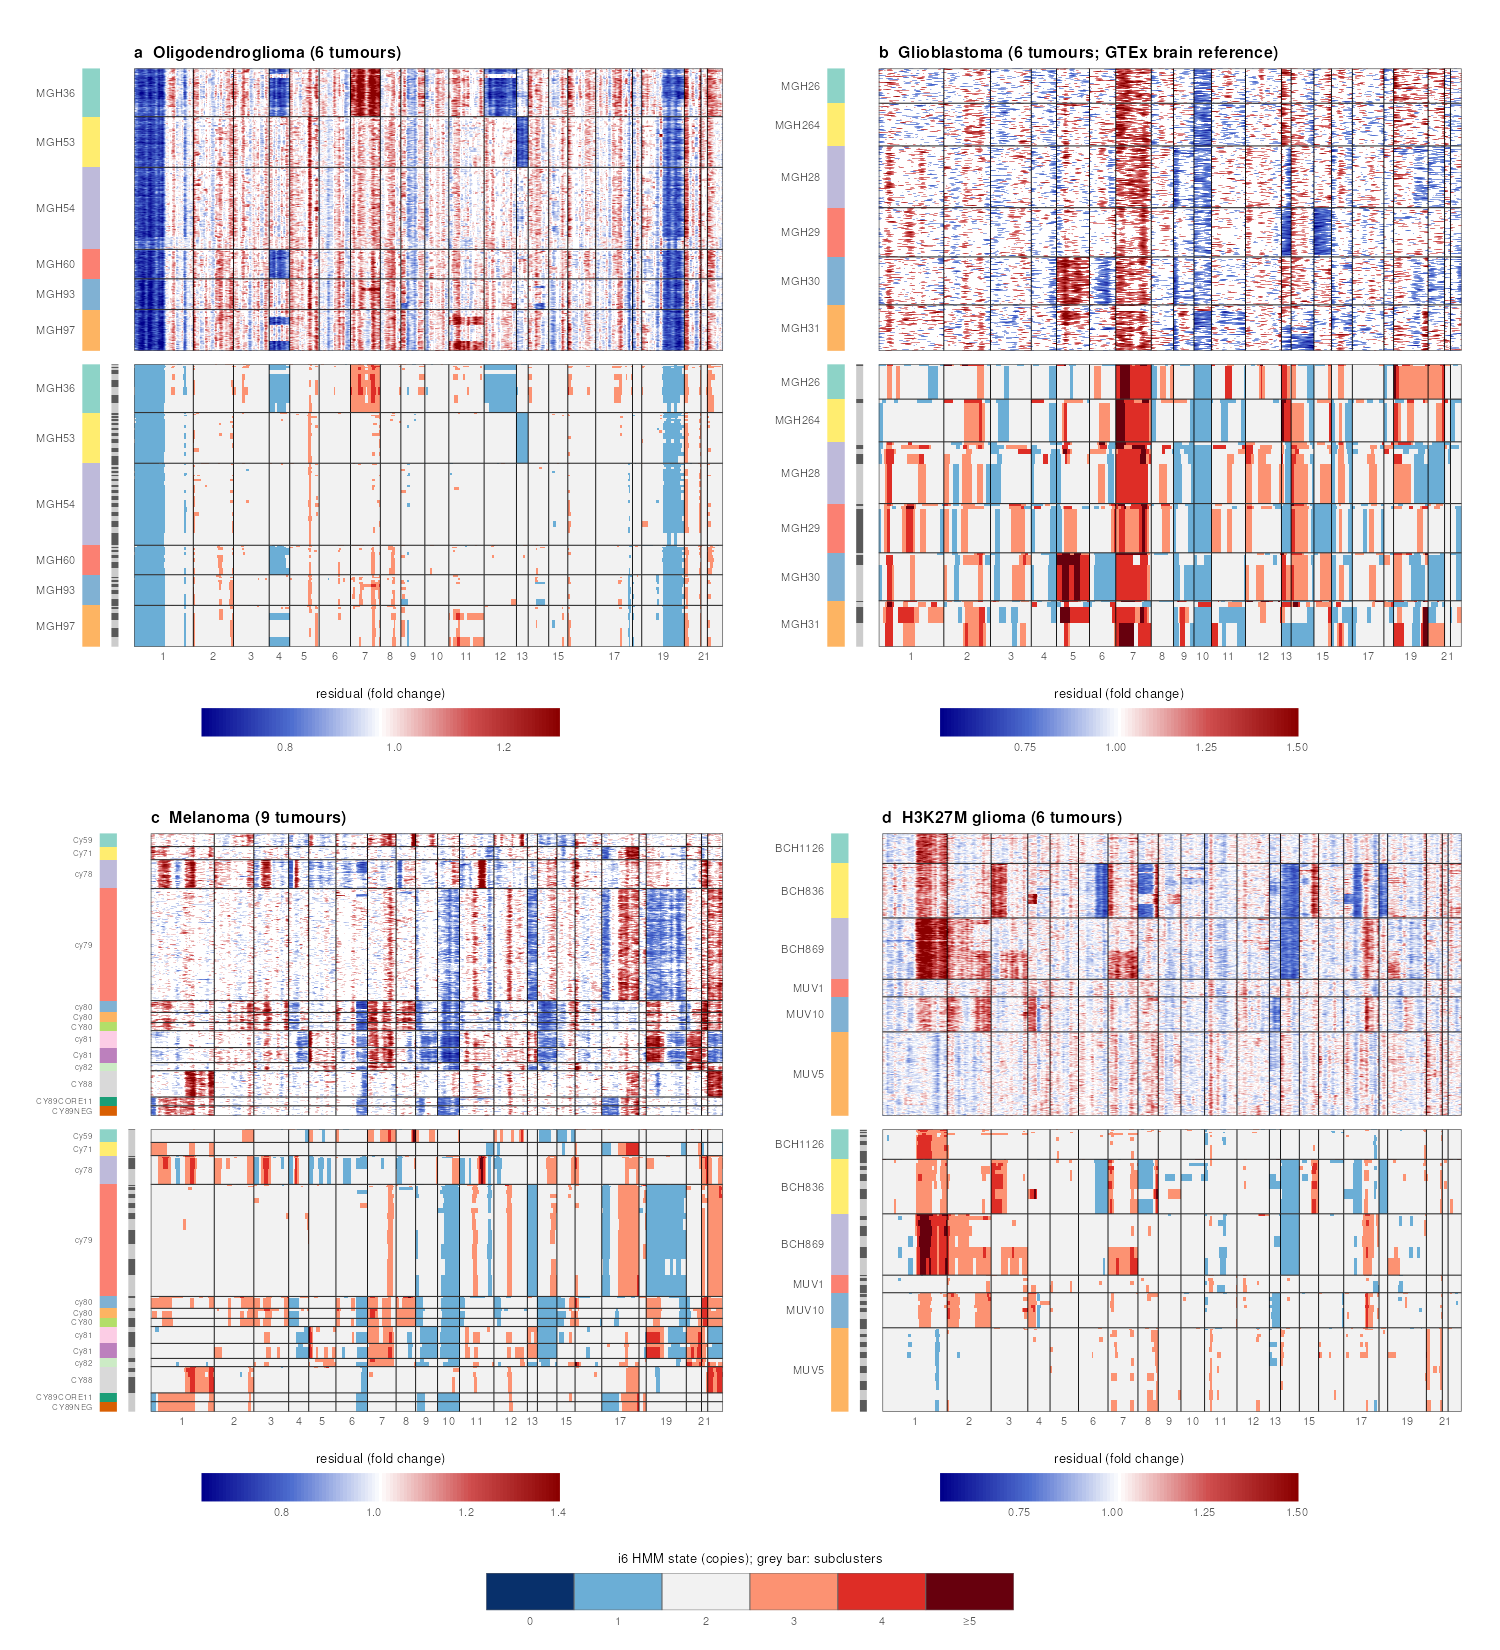
\includegraphics[width=\textwidth]{figures/fig3_gallery.png}
\caption{\textbf{inferCNV applied to tumours profiled with Smart-seq2.} Final residual expression of the malignant cells (top; fold-change scale) and i6 HMM states after Bayesian filtering (bottom) for (a) oligodendroglioma (six tumours, 4,043 cells), (b) glioblastoma (six tumours, 421 cells; reference: nine oligodendrocytes identified among the profiled cells), (c) melanoma (1,173 malignant cells from nine tumours; annotation labels differing only in case, or marking two samples of one tumour, were merged after their CNA profiles were found to correlate at 0.96--0.98) and (d) H3K27M glioma (six tumours, 2,259 cells), from the inferCNV\_examples data. Rows are cells grouped by tumour (coloured bar) and ordered by subcluster (alternating grey bar); reference cells are not shown.}
\label{fig:3}
\end{figure}}

% fig:subclusters
\expandafter\long\expandafter\def\csname float@fig:subclusters\endcsname{%
\begin{figure}[tbp]
\centering
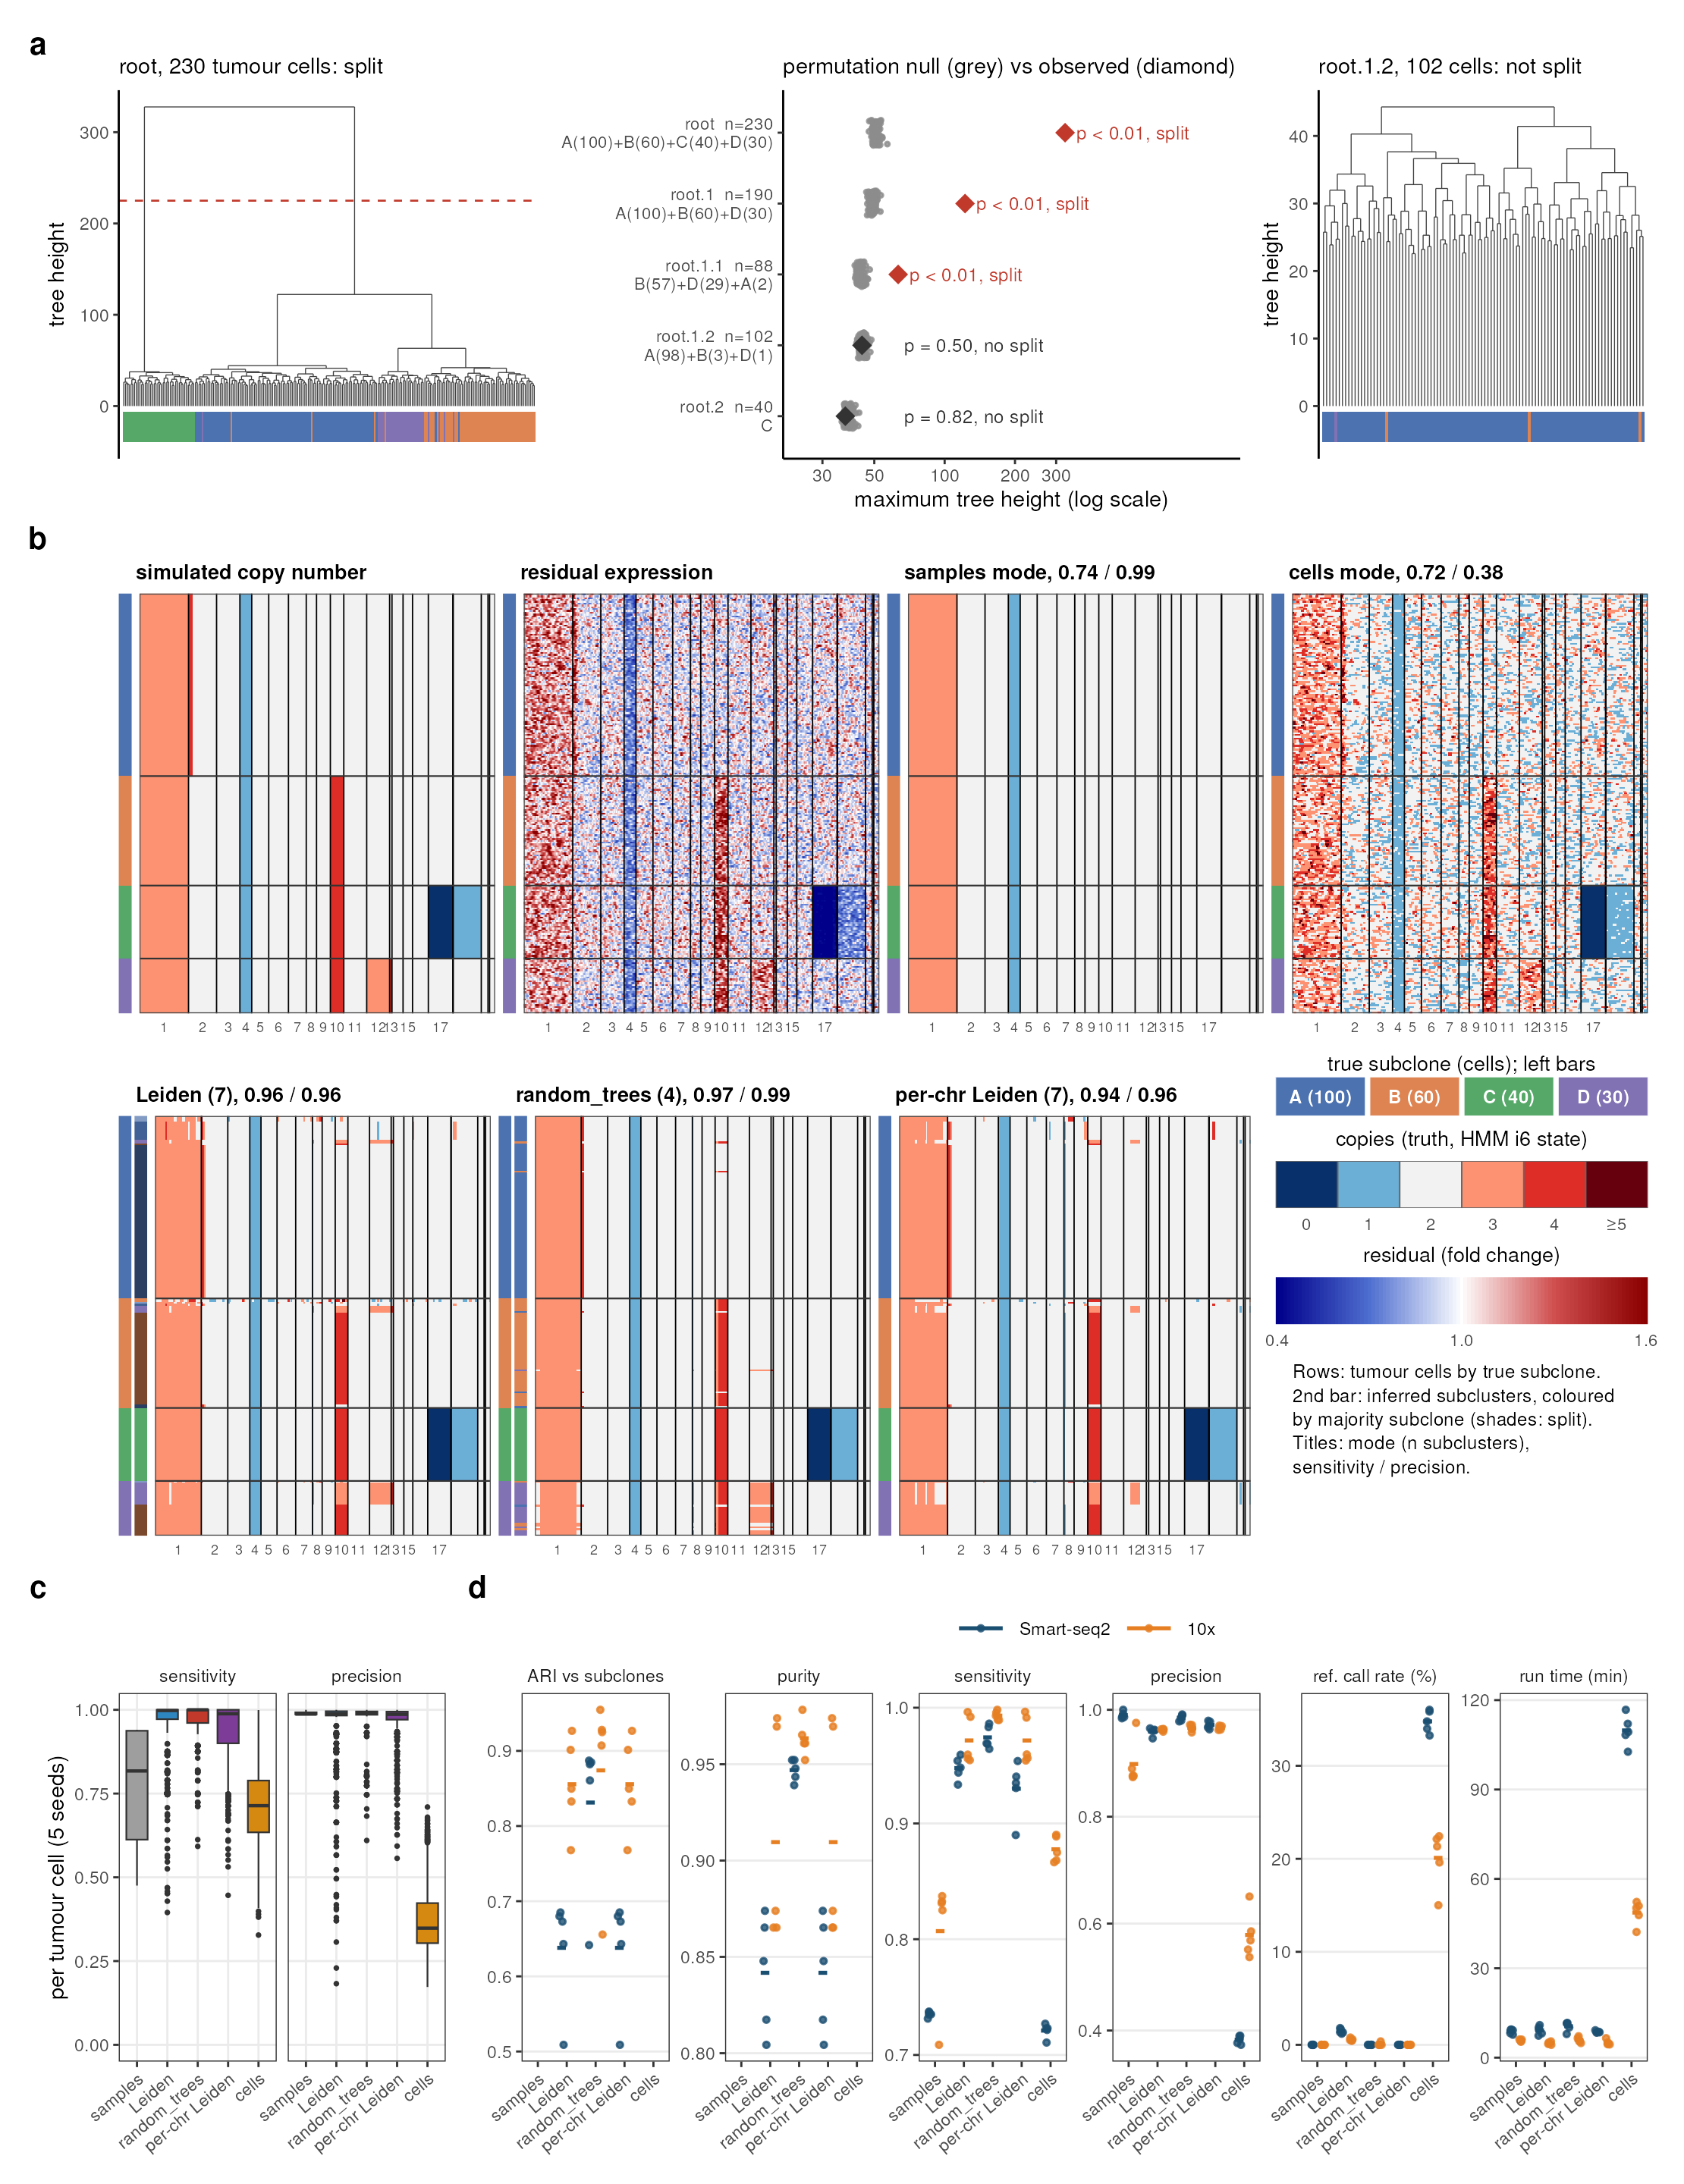
\includegraphics[width=\textwidth]{figures/fig_subclusters.png}
\caption{\textbf{Subclustering sets the resolution of the HMM.} Simulated Smart-seq2 tumour with four subclones, A--D (100, 60, 40 and 30 cells; sim4), and 100 reference cells, analysed as a single annotation group with the i6 HMM and the Bayesian filter. (a) \texttt{random\_trees} permutation test (seed 1). Left, \texttt{ward.D2} dendrogram of the 230 tumour cells, computed on smoothed residuals; the bar shows the true subclones and the dashed line the top split. Middle, maximum tree height at each node of the recursion (diamond) against its null from 100 permutations in which each gene's values are shuffled across cells (grey). Nodes are labelled with their size and true composition. A node is split when p $\leq$ 0.1 (\texttt{tumor\_subcluster\_pval}); recursion depth is limited to 3. Right, dendrogram of subclone A (root.1.2), which is not split (p = 0.50). (b) Simulated copy number, residual expression (fold change, before denoising) and i6 states after Bayesian filtering for each analysis mode. Rows are tumour cells ordered by true subclone (left bar). The second bar shows the inferred subclusters, coloured by their majority subclone; shades mark subclusters of the same subclone. The per-chromosome Leiden partitions are not shown. Titles give the number of tumour subclusters and the cell $\times$ gene sensitivity / precision. Colour bar: i6 state as copies (0, 1, 2, 3, 4, $\geq$5). (c) Per-cell sensitivity and precision of tumour cells for each mode (Smart-seq2, five seeds). (d) Summary over five seeds (points) with means (bars) for Smart-seq2 and 10x: ARI and purity of the tumour subclusters against the true subclones; cell $\times$ gene sensitivity and precision; non-neutral call rate in reference cells; run time with 4 threads.}
\label{fig:subclusters}
\end{figure}}

% fig:4
\expandafter\long\expandafter\def\csname float@fig:4\endcsname{%
\begin{figure}[tbp]
\centering
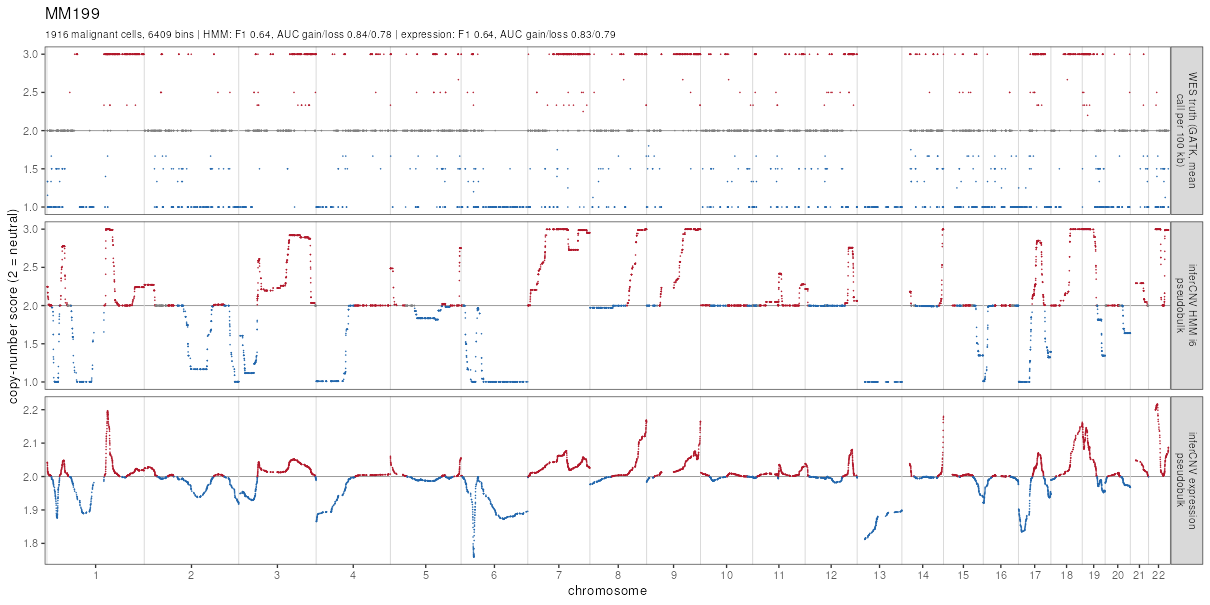
\includegraphics[width=\textwidth]{figures/fig4_MM199_genome.png}\\[1ex]
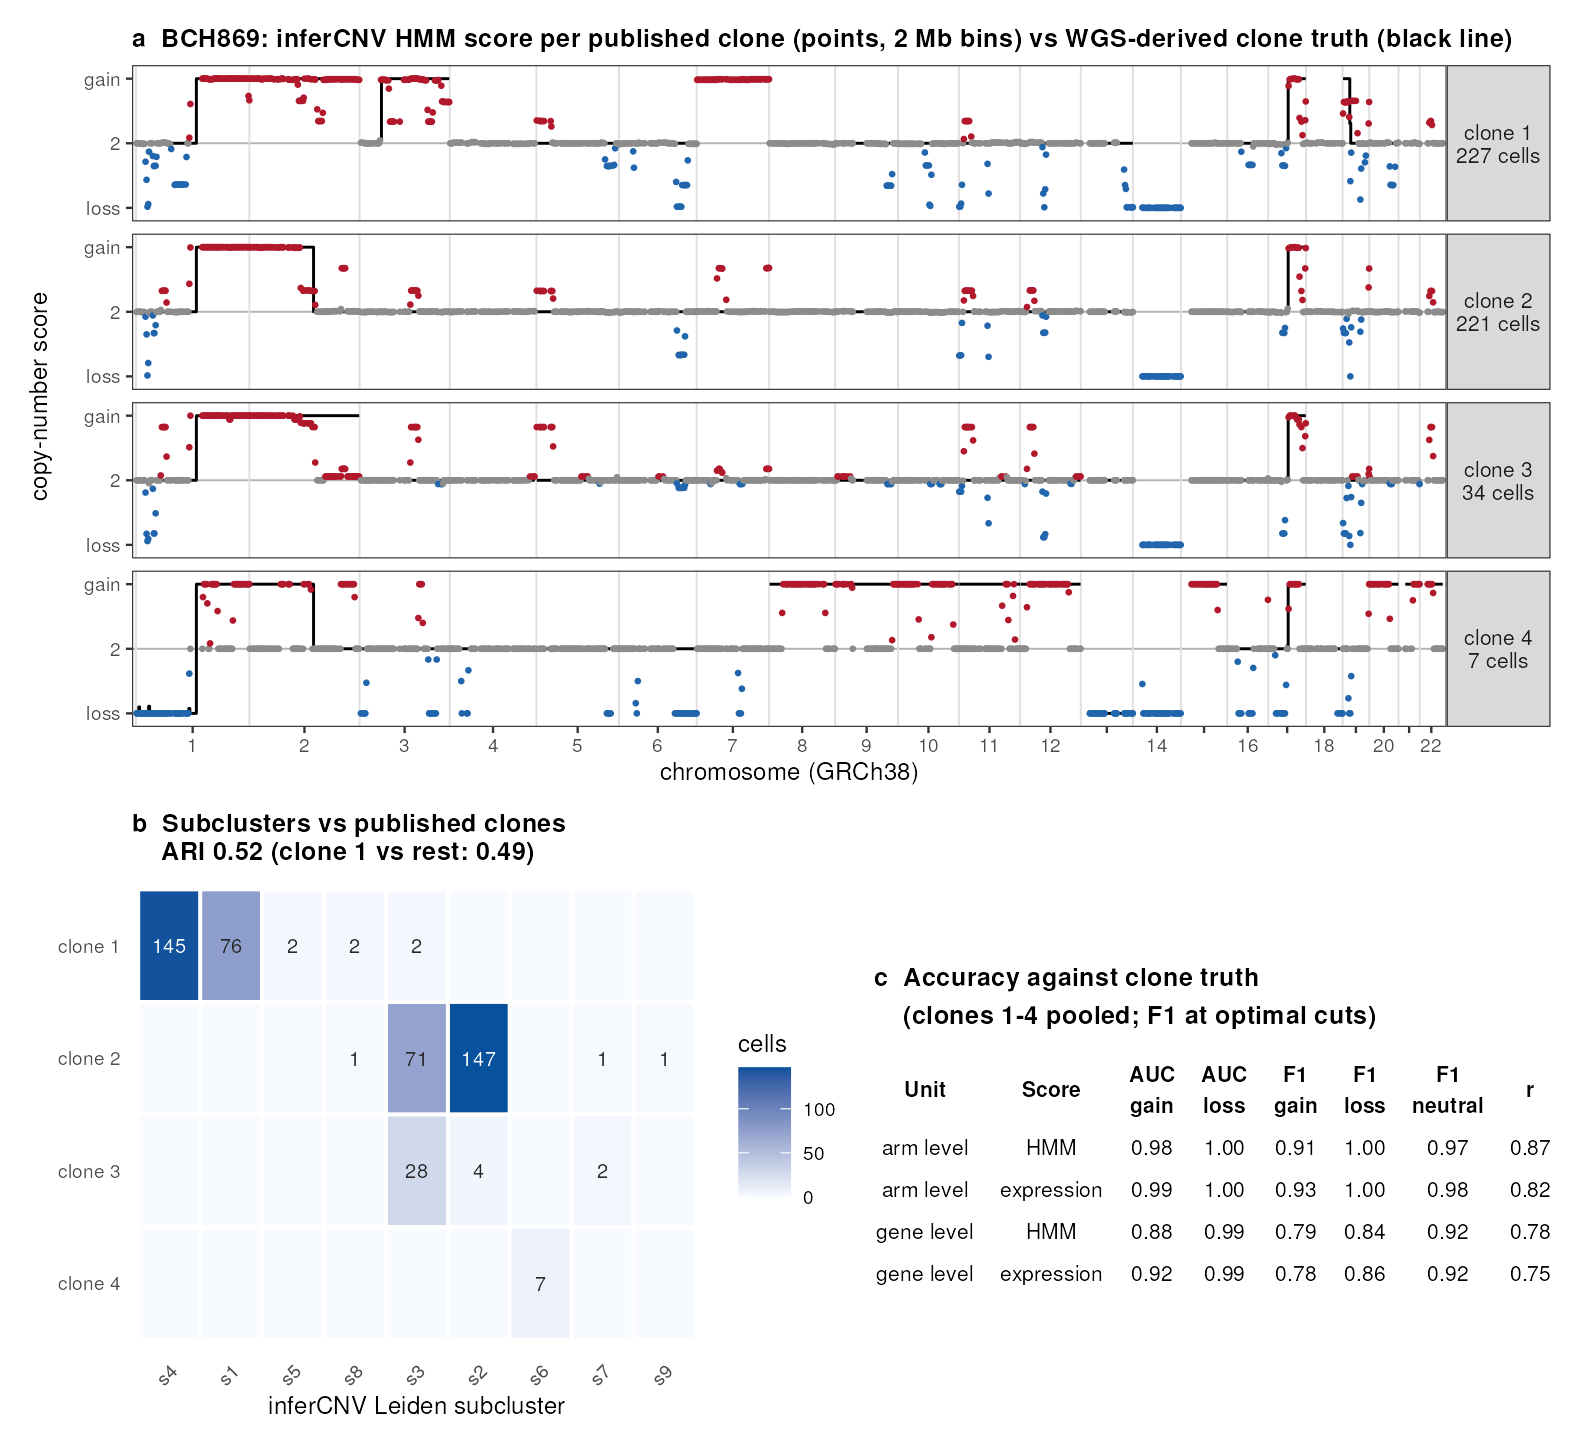
\includegraphics[width=0.92\textwidth]{figures/fig4_BCH869.png}
\caption{\textbf{Comparison with DNA-based copy number.} \textbf{a}, Multiple myeloma MM199 (10x). Top, whole-exome copy number segments (Schmid et al.~truth). Below, inferCNV pseudobulk scores over 1,916 malignant cells: HMM states after Bayesian filtering (CNV score) and final residual expression (expression score), in 100-kb bins along the genome. \textbf{b}, H3K27M glioma BCH869 (Smart-seq2; published TPM matrix, hg19 gene positions). Top, inferCNV pseudobulk HMM score (i6 states after Bayesian filtering, mean over cells) for each published clone in 2-Mb bins (points), with the clone's copy number derived from whole-genome sequencing (black line) \citep{filbin2018, huang2024xclone}. The reference was the immune and oligodendrocyte cells of a second tumour, BCH1126, one group per cell type. Bottom left, cells of each published clone across inferCNV's Leiden subclusters; bottom right, AUC and F1 for gains and losses at chromosome-arm and gene level, clones pooled. Settings as in Methods.}
\label{fig:4}
\end{figure}}

% fig:5
\expandafter\long\expandafter\def\csname float@fig:5\endcsname{%
\begin{figure}[tbp]
\centering
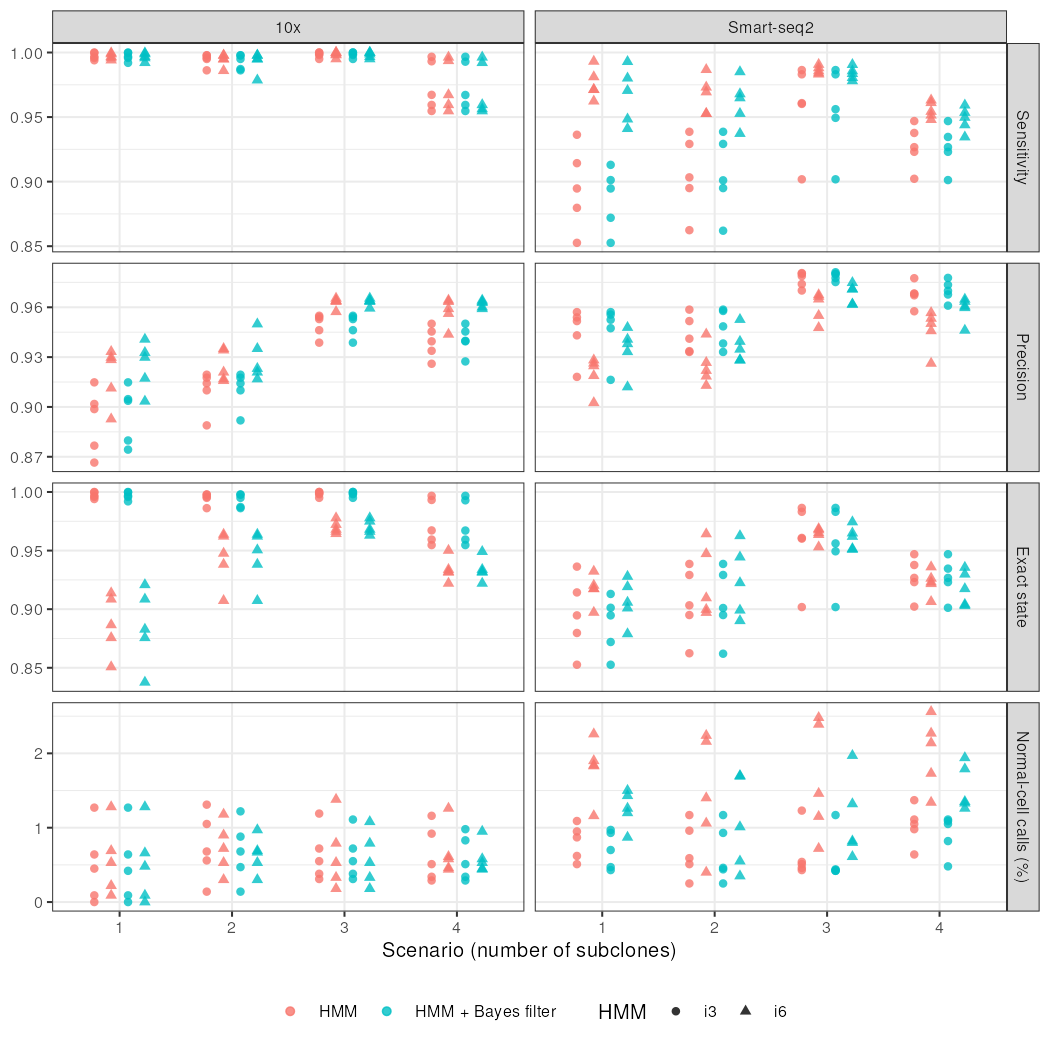
\includegraphics[width=\textwidth]{figures/fig5_simulation.png}
\caption{\textbf{Accuracy on simulated tumours.} Cell $\times$ gene sensitivity, precision, exact-state accuracy and the non-neutral call rate in reference cells, for simulated 10x and Smart-seq2 tumours with one to four subclones (sim1--sim4), with the i6 (triangles) and i3 (circles) HMM, before (red) and after (blue) Bayesian filtering. Each point is one of five simulation seeds. Mean values for i6 after filtering, and subcluster purity, are in Table~1.}
\label{fig:5}
\end{figure}}

% fig:6
\expandafter\long\expandafter\def\csname float@fig:6\endcsname{%
\begin{figure}[tbp]
\centering
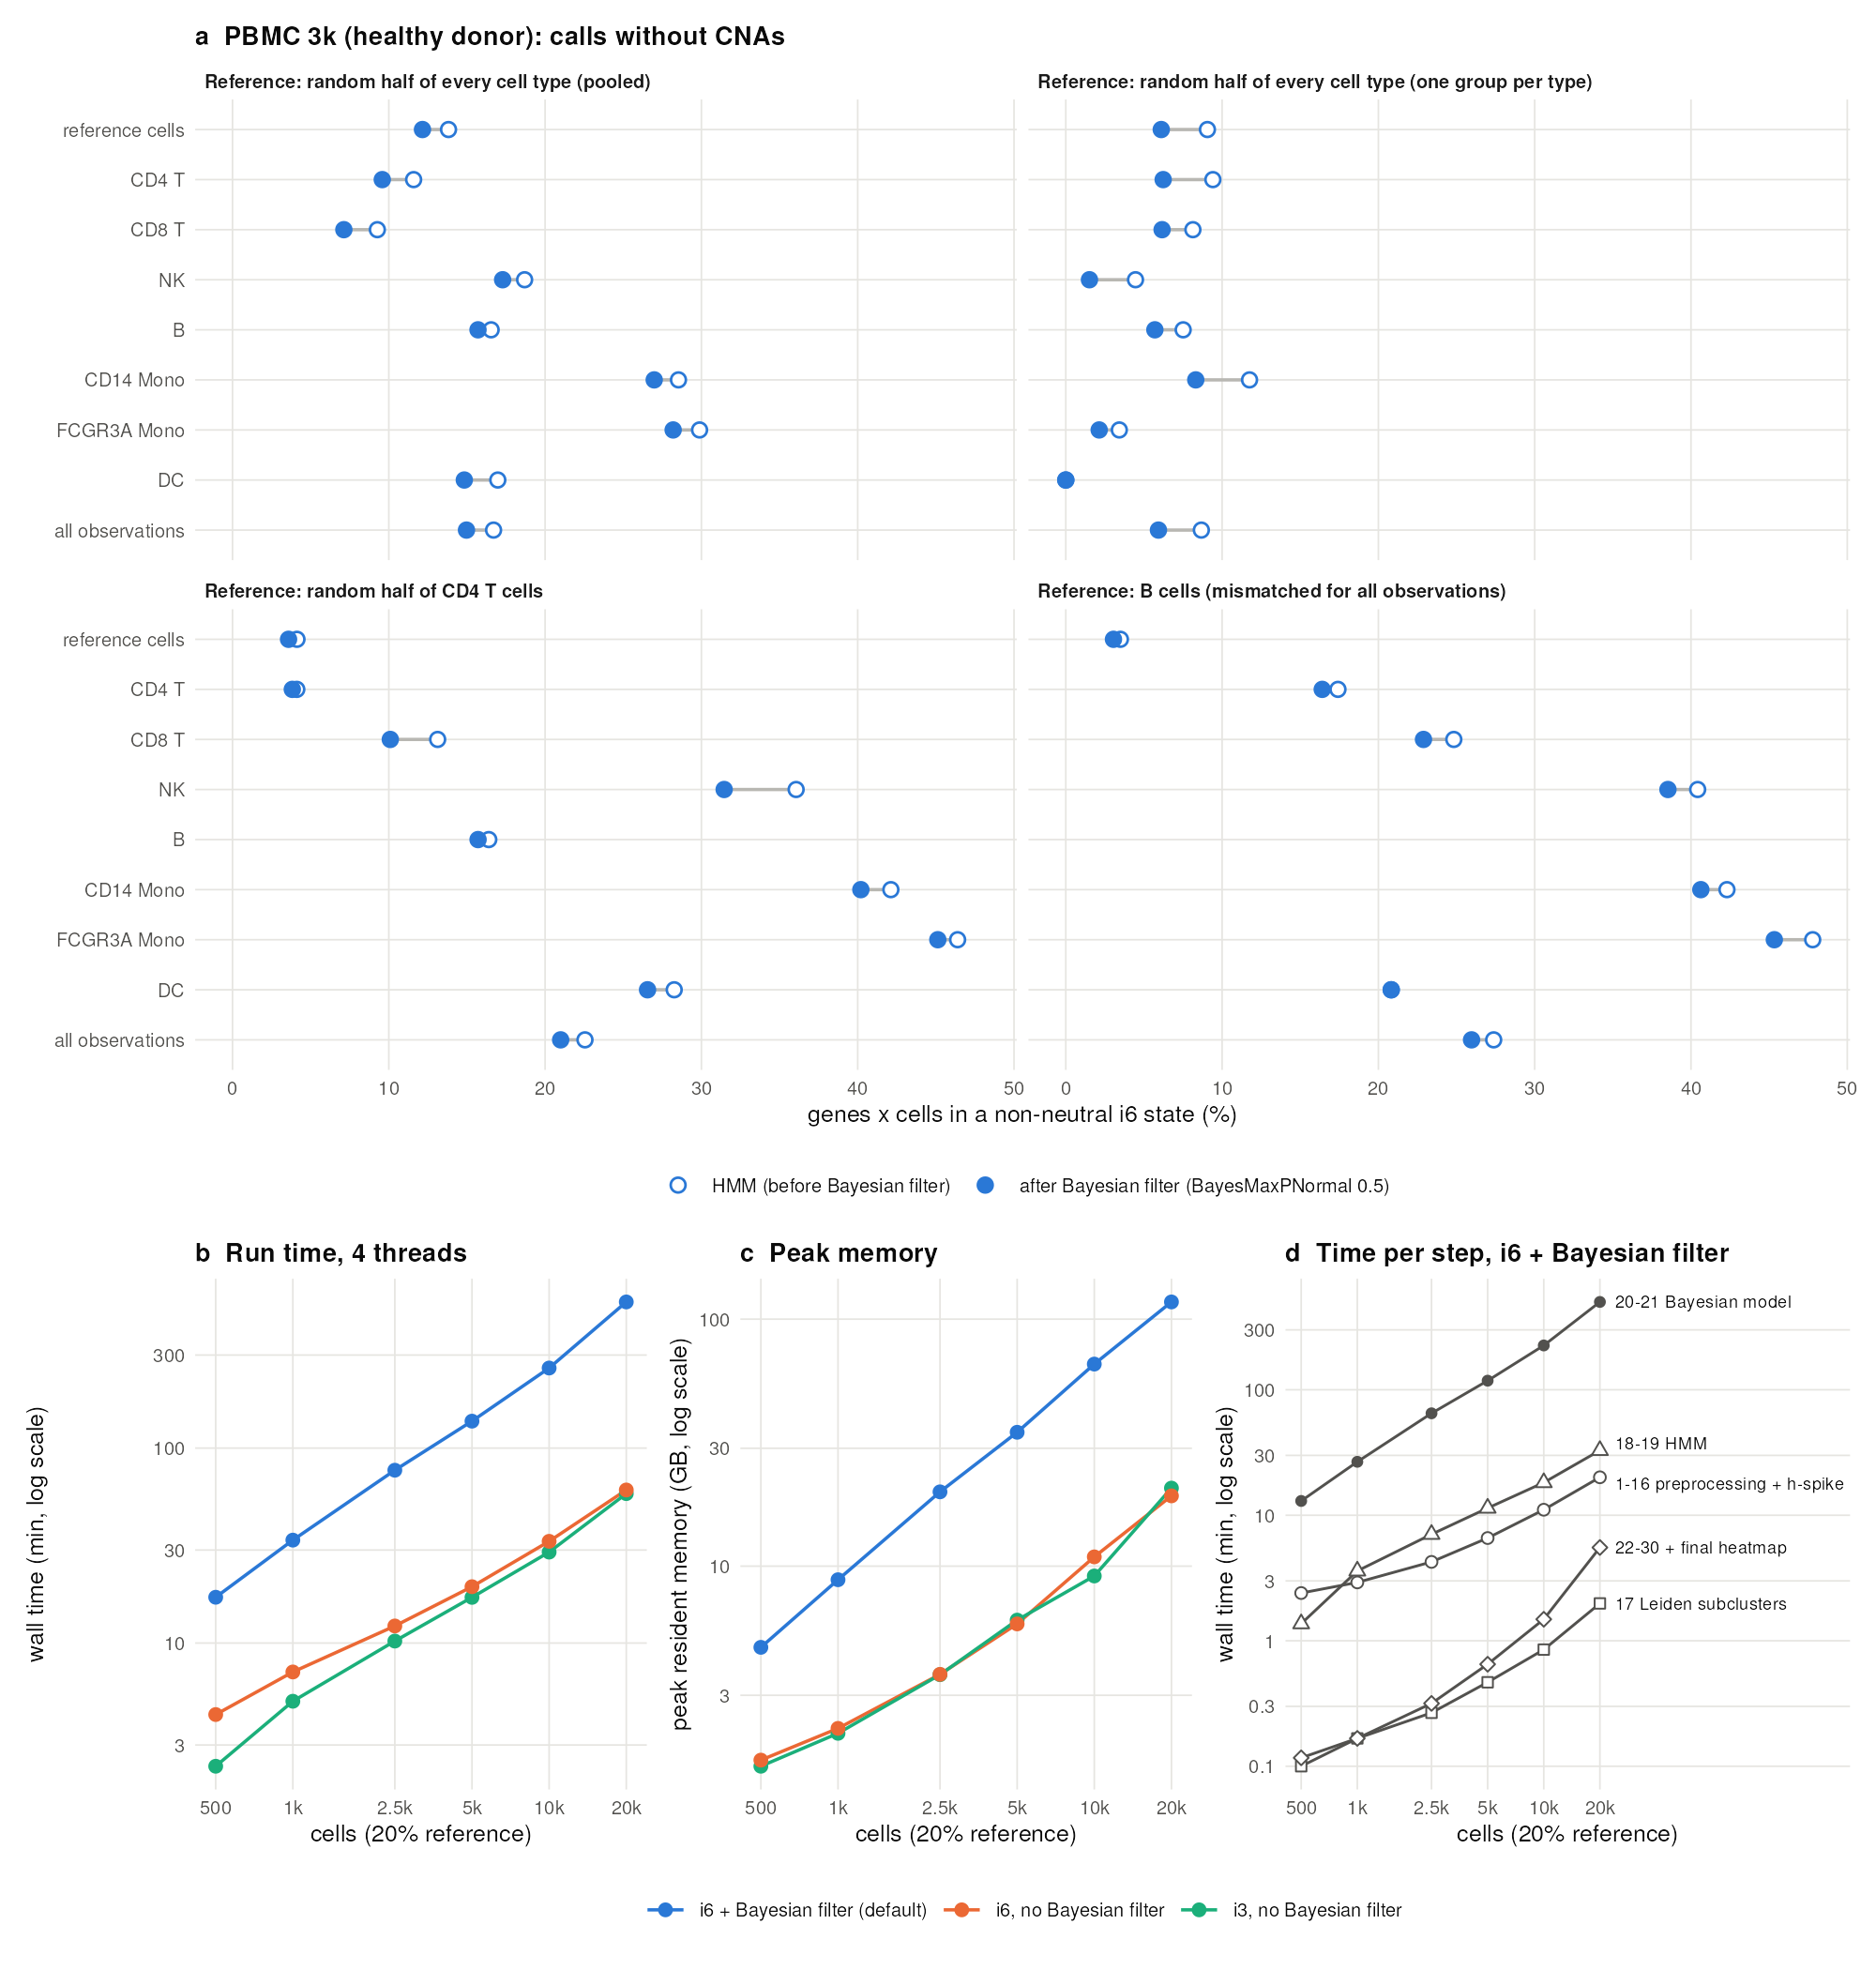
\includegraphics[width=\textwidth]{figures/fig6_specificity_scaling.png}
\caption{\textbf{Specificity and scale.} (a) Fraction of genes $\times$ cells in a non-neutral i6 state in PBMC from a healthy donor (10x, 2,625 cells), which carry no CNAs, by cell type, before (open) and after (filled) Bayesian filtering, for four reference designs: a random half of every cell type as the reference, pooled into one group or given as one group per cell type; a random half of the CD4 T cells; and all B cells. ``Reference cells'' shows the calls in the reference cells themselves. (b) Wall time and (c) peak resident memory against the number of cells (nested down-samples of a 10x breast cancer atlas, 20\% reference cells, 4 threads) for i6 with the Bayesian filter (default), i6 without it, and i3 without it. (d) Time per step of the default run; the Bayesian model dominates.}
\label{fig:6}
\end{figure}}

% fig:7
\expandafter\long\expandafter\def\csname float@fig:7\endcsname{%
\begin{figure}[tbp]
\centering
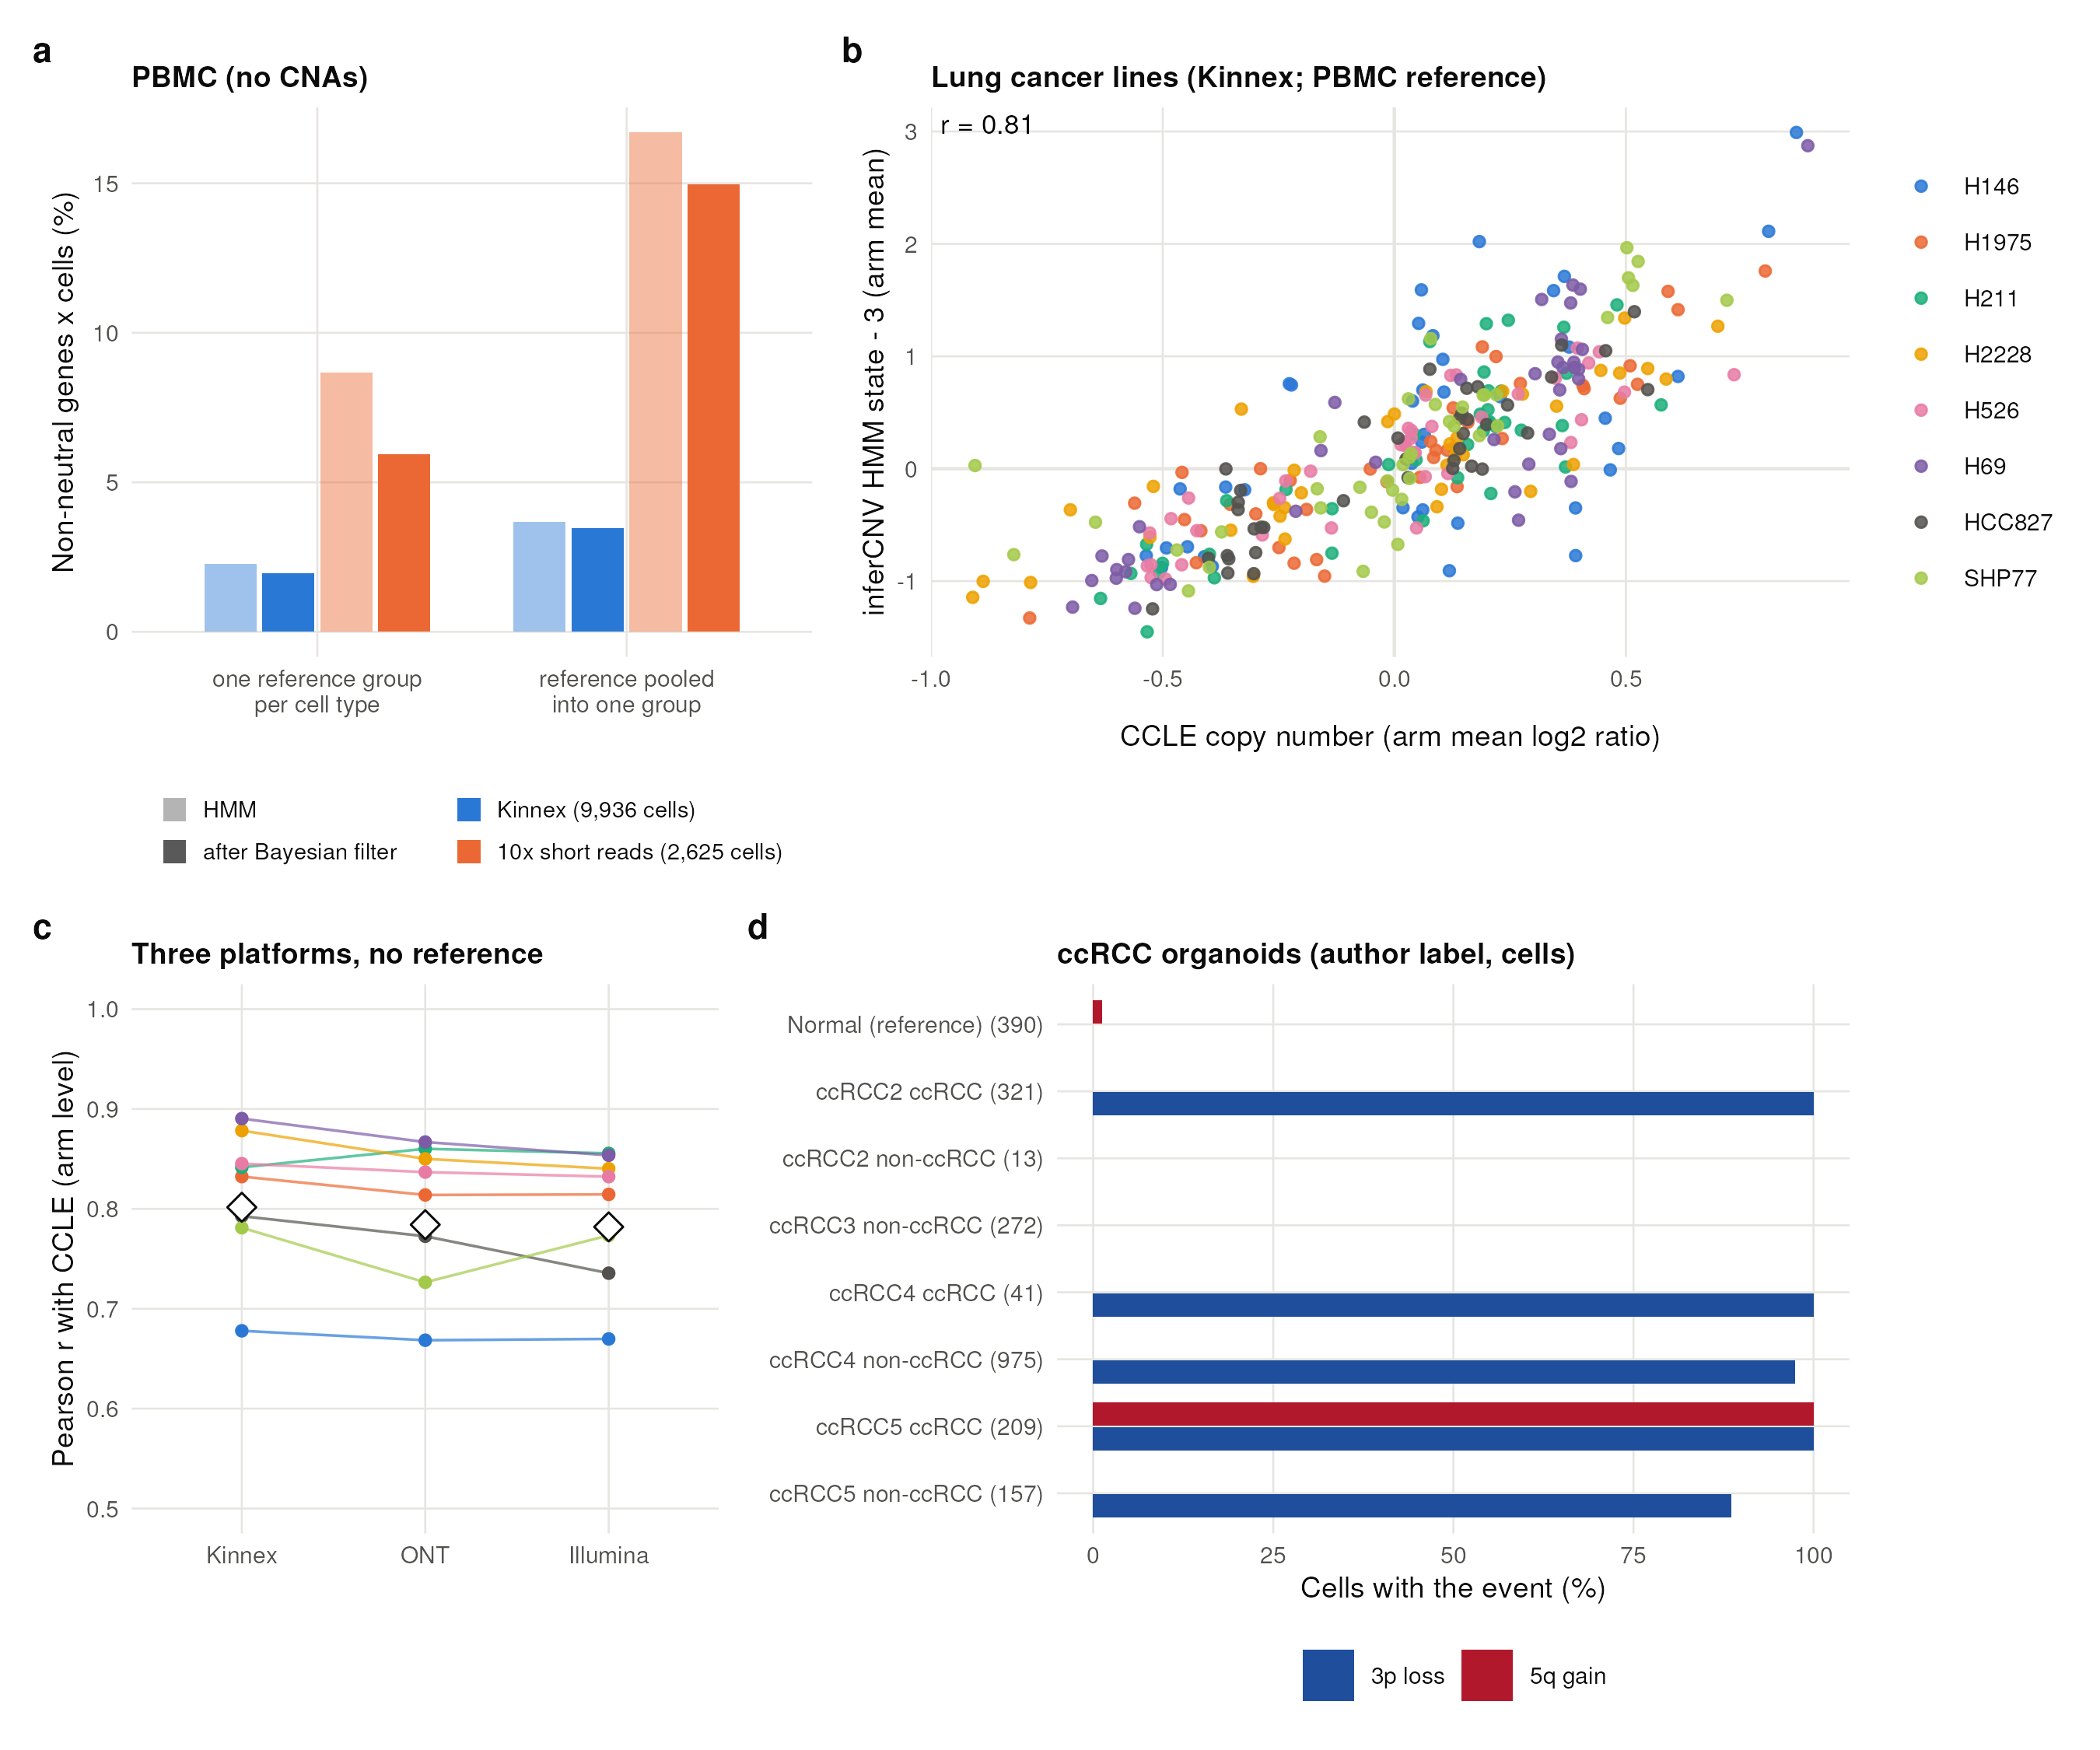
\includegraphics[width=\textwidth]{figures/fig7_longread.png}
\caption{\textbf{Long-read single-cell data.} (a) Fraction of genes $\times$ cells in a non-neutral i6 state in PBMC without CNAs, for Kinnex long reads (9,936 cells) and the 10x short-read data of Fig.~\ref{fig:6}a (2,625 cells), with a random half of every cell type as the reference, given as one group per cell type or pooled; light bars, HMM; dark bars, after Bayesian filtering. (b) Eight lung cancer cell lines (LongBench, Kinnex, 3,850 cells) analysed with the Kinnex PBMCs as the reference: mean HMM state per chromosome arm, relative to neutral, against CCLE copy number (mean log$_2$ ratio); one point per line and arm. (c) Pearson correlation with CCLE per line (coloured) and pooled (diamonds) for the same cells sequenced with Kinnex, ONT and Illumina and analysed without a reference (CCLE values centred on the mean of the lines). (d) ccRCC patient-derived organoids (MAS-ISO-seq) analysed with a normal kidney organoid as the reference: percentage of cells with 3p loss and with 5q gain by organoid and by the original authors' expression-based label (cell numbers in parentheses).}
\label{fig:7}
\end{figure}}

% fig:8
\expandafter\long\expandafter\def\csname float@fig:8\endcsname{%
\begin{figure}[tbp]
\centering
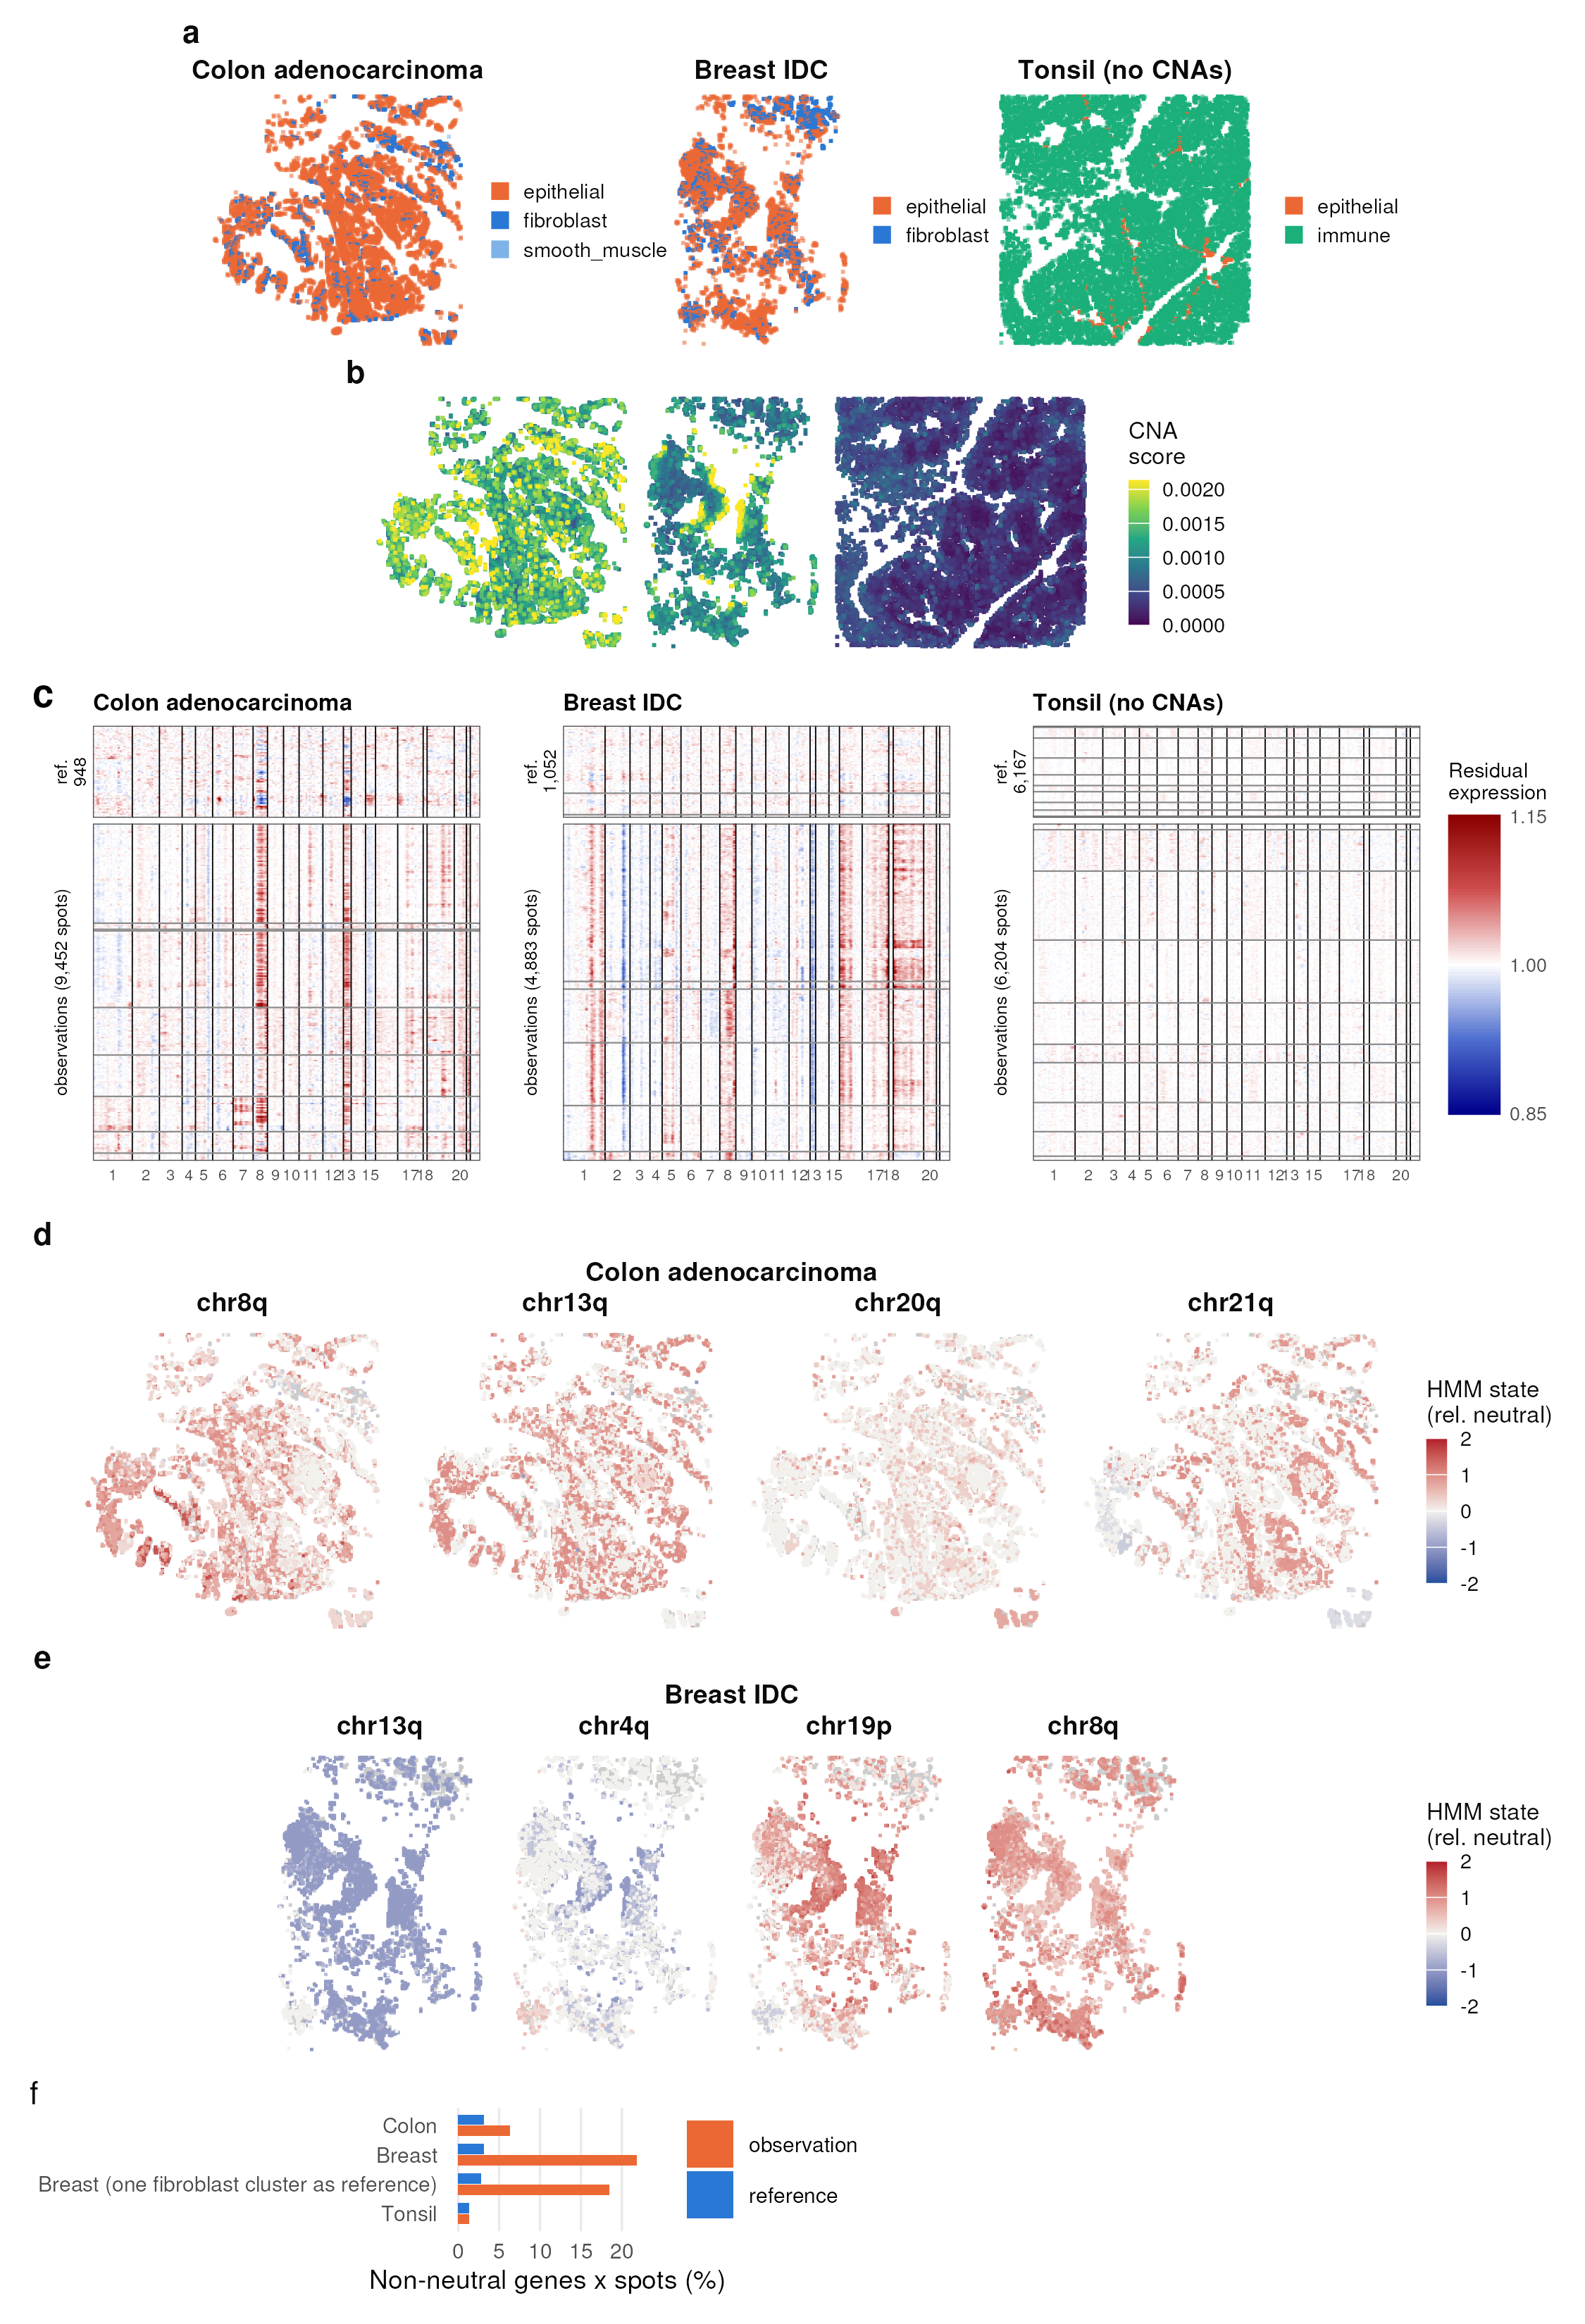
\includegraphics[width=\textwidth]{figures/fig8_visiumhd.png}
\caption{\textbf{Spatial long-read data (Kinnex Visium HD).} Sections of a colon adenocarcinoma, a breast infiltrating ductal carcinoma and a tonsil, summed into 32-\textmu m spots with at least 1,000 counts. (a) Tissue compartments from marker scores of spot clusters; reference spots are shown in full colour. In the tumours, fibroblast spots were the reference for epithelial spots; in the tonsil, which serves as a control without CNAs, half of each cluster was the reference for the other half. (b) CNA score (mean squared residual expression), on a common scale. (c) Genome-wide inferCNV residual expression (chromosomes 1--22) of the reference spots (top) and observation spots (bottom) of each section, on a common colour scale; spots are ordered by cluster (grey lines) and, within clusters, by subcluster, and rows and genes are averaged in blocks for display. (d, e) Mean HMM state, relative to neutral, of each spot's inferCNV subcluster over selected chromosome arms in the colon (d) and breast (e) tumours; reference spots in grey. (f) Fraction of genes $\times$ spots in a non-neutral i6 state (HMM without Bayesian filter) in observation and reference spots, including the breast tumour analysed with a single fibroblast cluster as the reference.}
\label{fig:8}
\end{figure}}

% fig:9
\expandafter\long\expandafter\def\csname float@fig:9\endcsname{%
\begin{figure}[tbp]
\centering
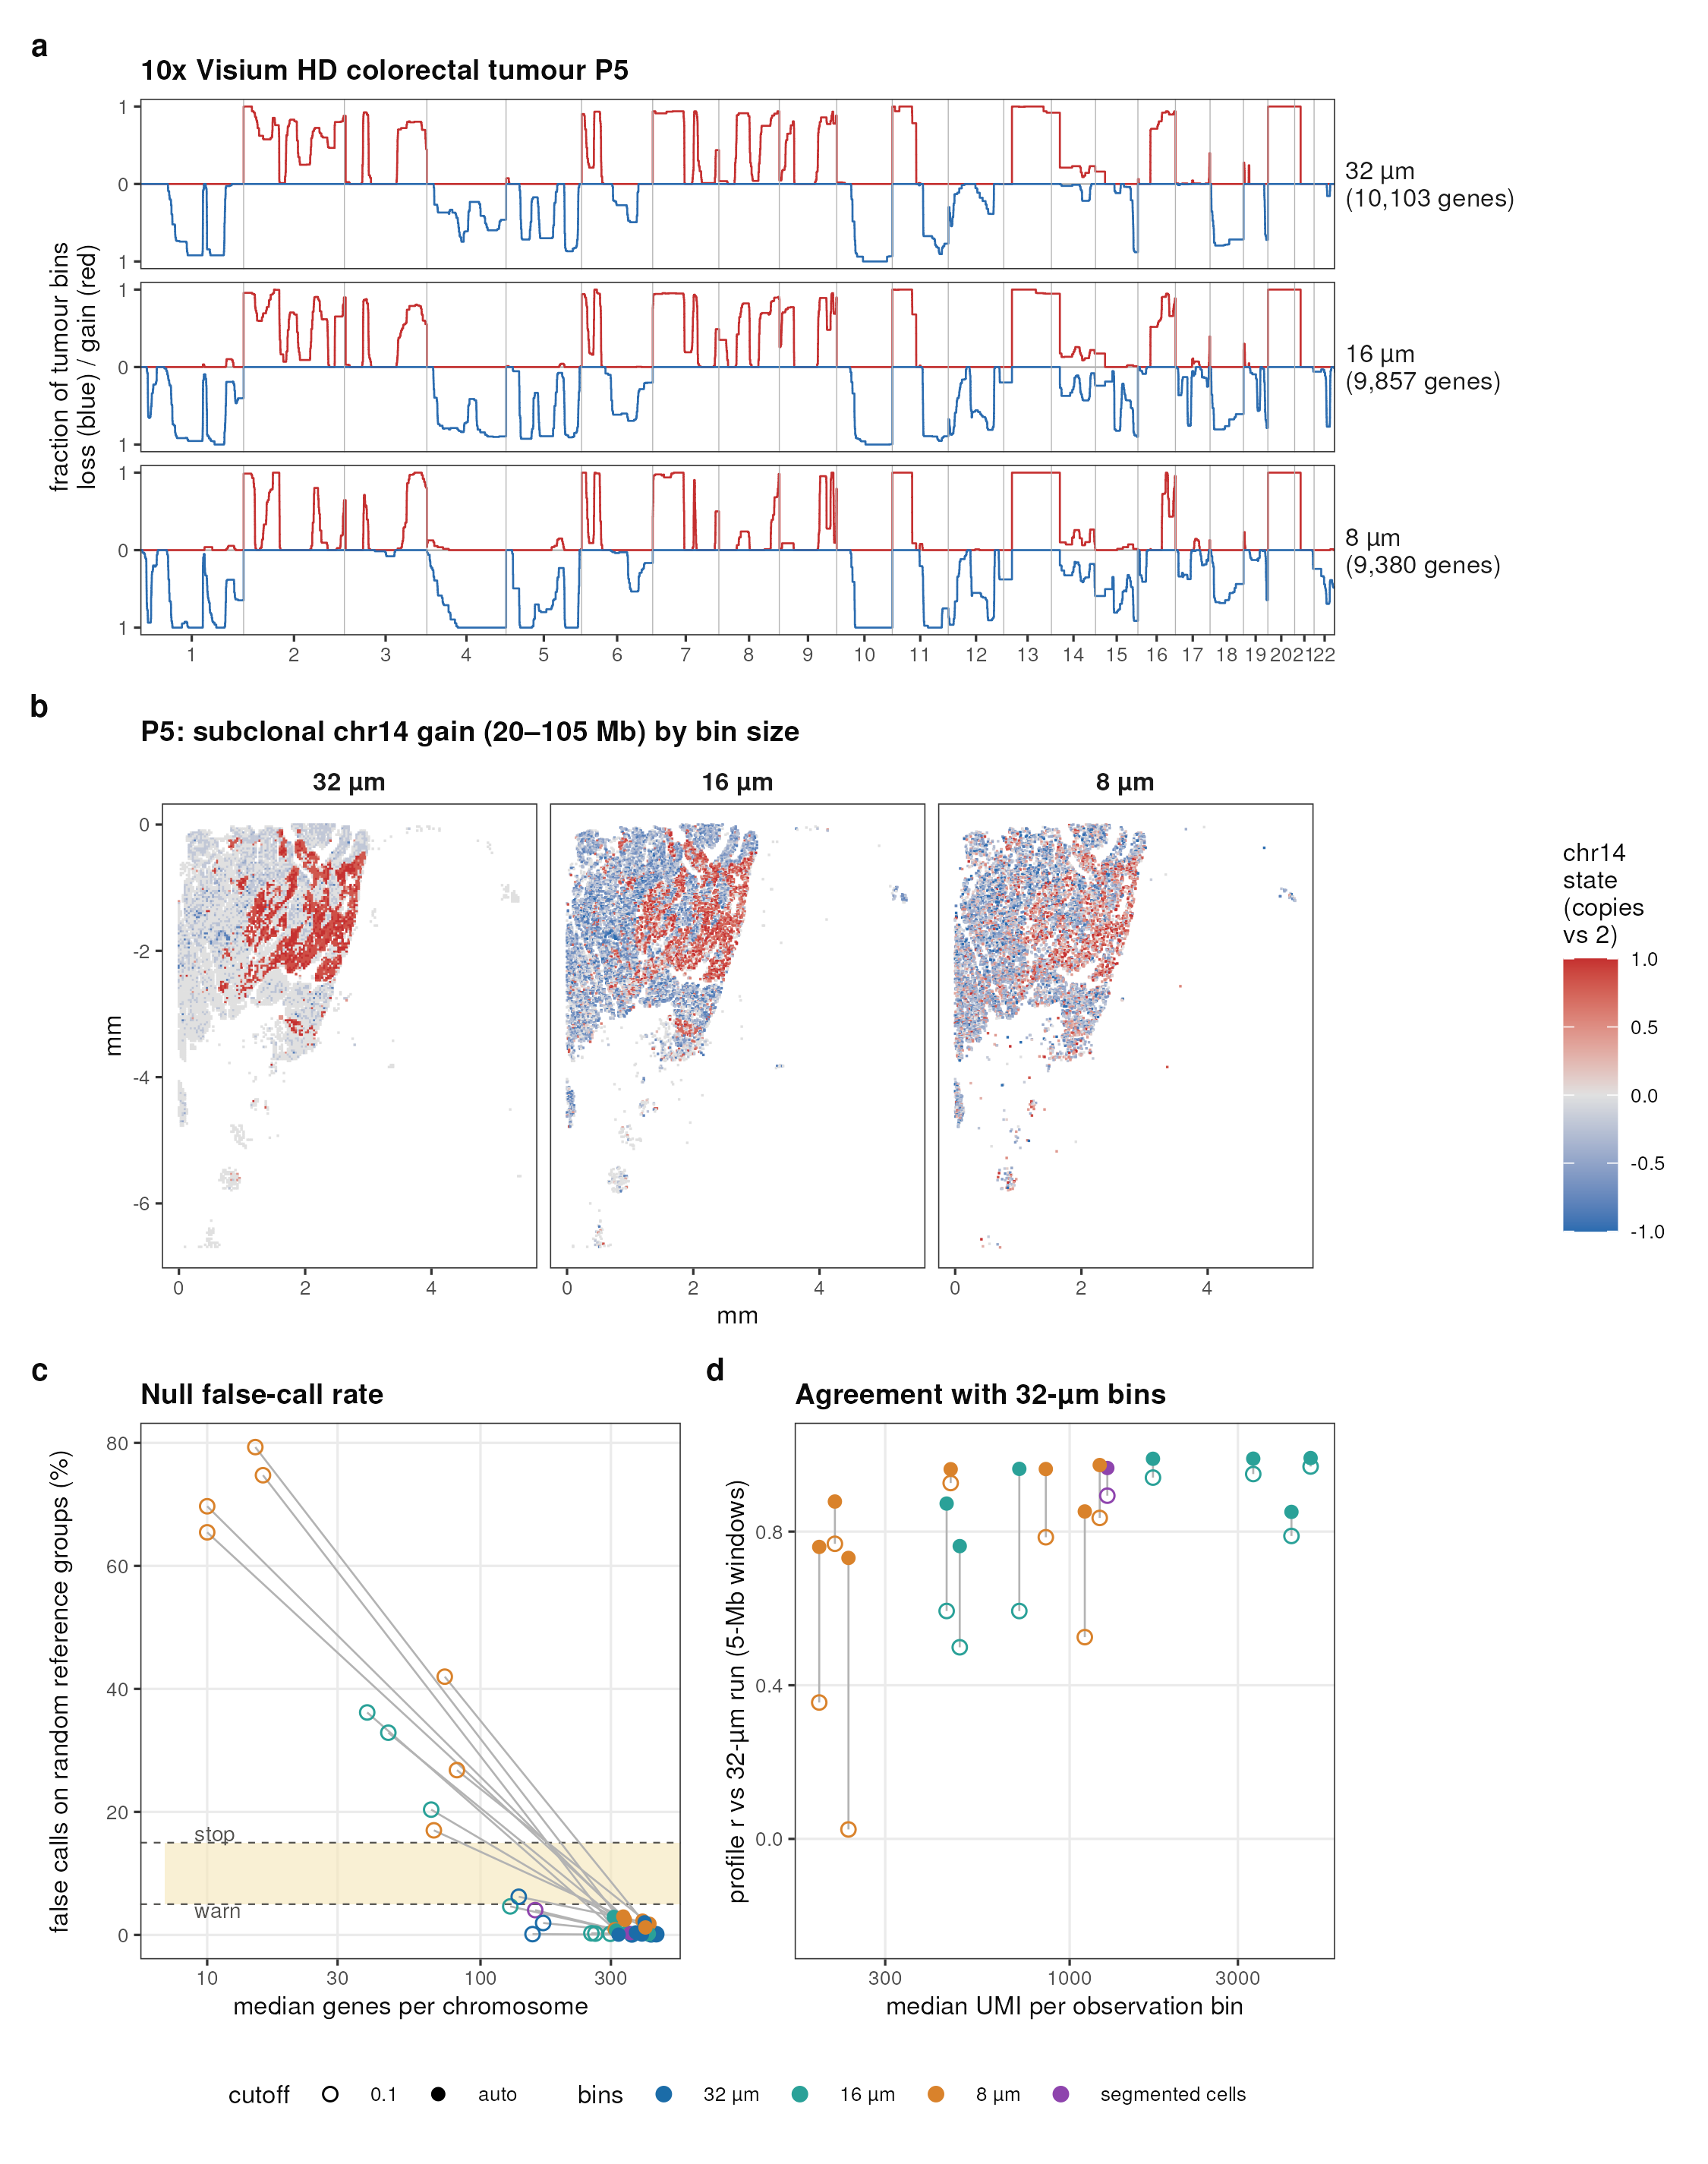
\includegraphics[width=\textwidth]{figures/fig9_resolution.png}
\caption{\textbf{Bin size, gene density and reliability of HMM calls in Visium HD data.} All runs use the default \texttt{cutoff\ =\ "auto"} unless stated. (a) 10x Visium HD colorectal tumour P5 at 32-, 16- and 8-\textmu m bins: fraction of tumour bins called gain (red, up) or loss (blue, down) by the HMM along chromosomes 1--22, with the number of genes kept. (b) Mean HMM state, relative to two copies, over chromosome 14 (20--105~Mb) for each tumour bin of P5. A gain of chromosome 14 defines a subclone at each bin size. (c) Null false-call rate (the fraction of genes $\times$ bins called in random groups of reference bins; \texttt{HMM\_null\_fpr\_check}) against the median number of genes per chromosome after the expression filter, at a cutoff of 0.1 (open) and at \texttt{"auto"} (filled), for 22 runs: 10x tumours P1, P2 and P5, 10x normal colon P3, and Kinnex colon, breast and tonsil, at three bin sizes, and P2 segmented cells. Lines join the two runs of each data set; dashed lines mark the warning (5\%) and stop (15\%) thresholds. (d) Correlation of each run's tumour (or epithelial) residual profile with the 32-\textmu m run of the same section, over 5-Mb windows, against the median count per observation bin, at the two cutoffs.}
\label{fig:9}
\end{figure}}

% fig:S1
\expandafter\long\expandafter\def\csname float@fig:S1\endcsname{%
\begin{figure}[p]
\centering
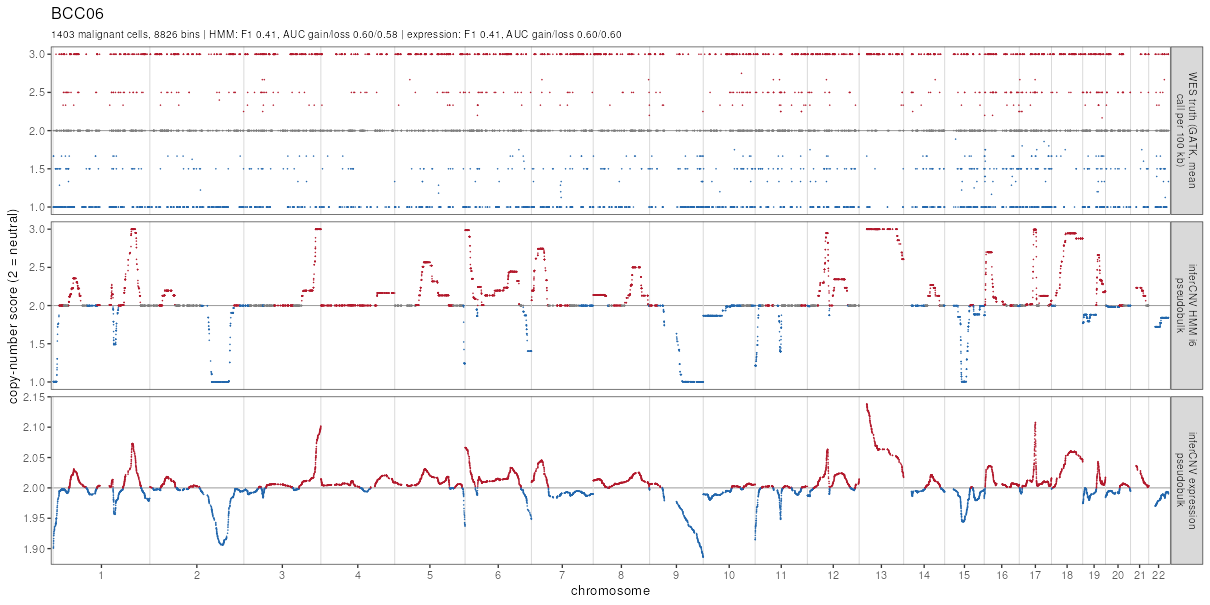
\includegraphics[width=\textwidth]{figures/figS1_BCC06_genome.png}
\caption{\textbf{Basal cell carcinoma BCC06 before and after treatment.} As Fig.~\ref{fig:4}, for BCC06 (1,403 malignant and 33 reference cells) and BCC06post (320 malignant and 280 reference cells). The exome segmentation of these samples is highly fragmented; see text.}
\label{fig:S1}
\end{figure}}

% fig:S2
\expandafter\long\expandafter\def\csname float@fig:S2\endcsname{%
\begin{figure}[p]
\centering
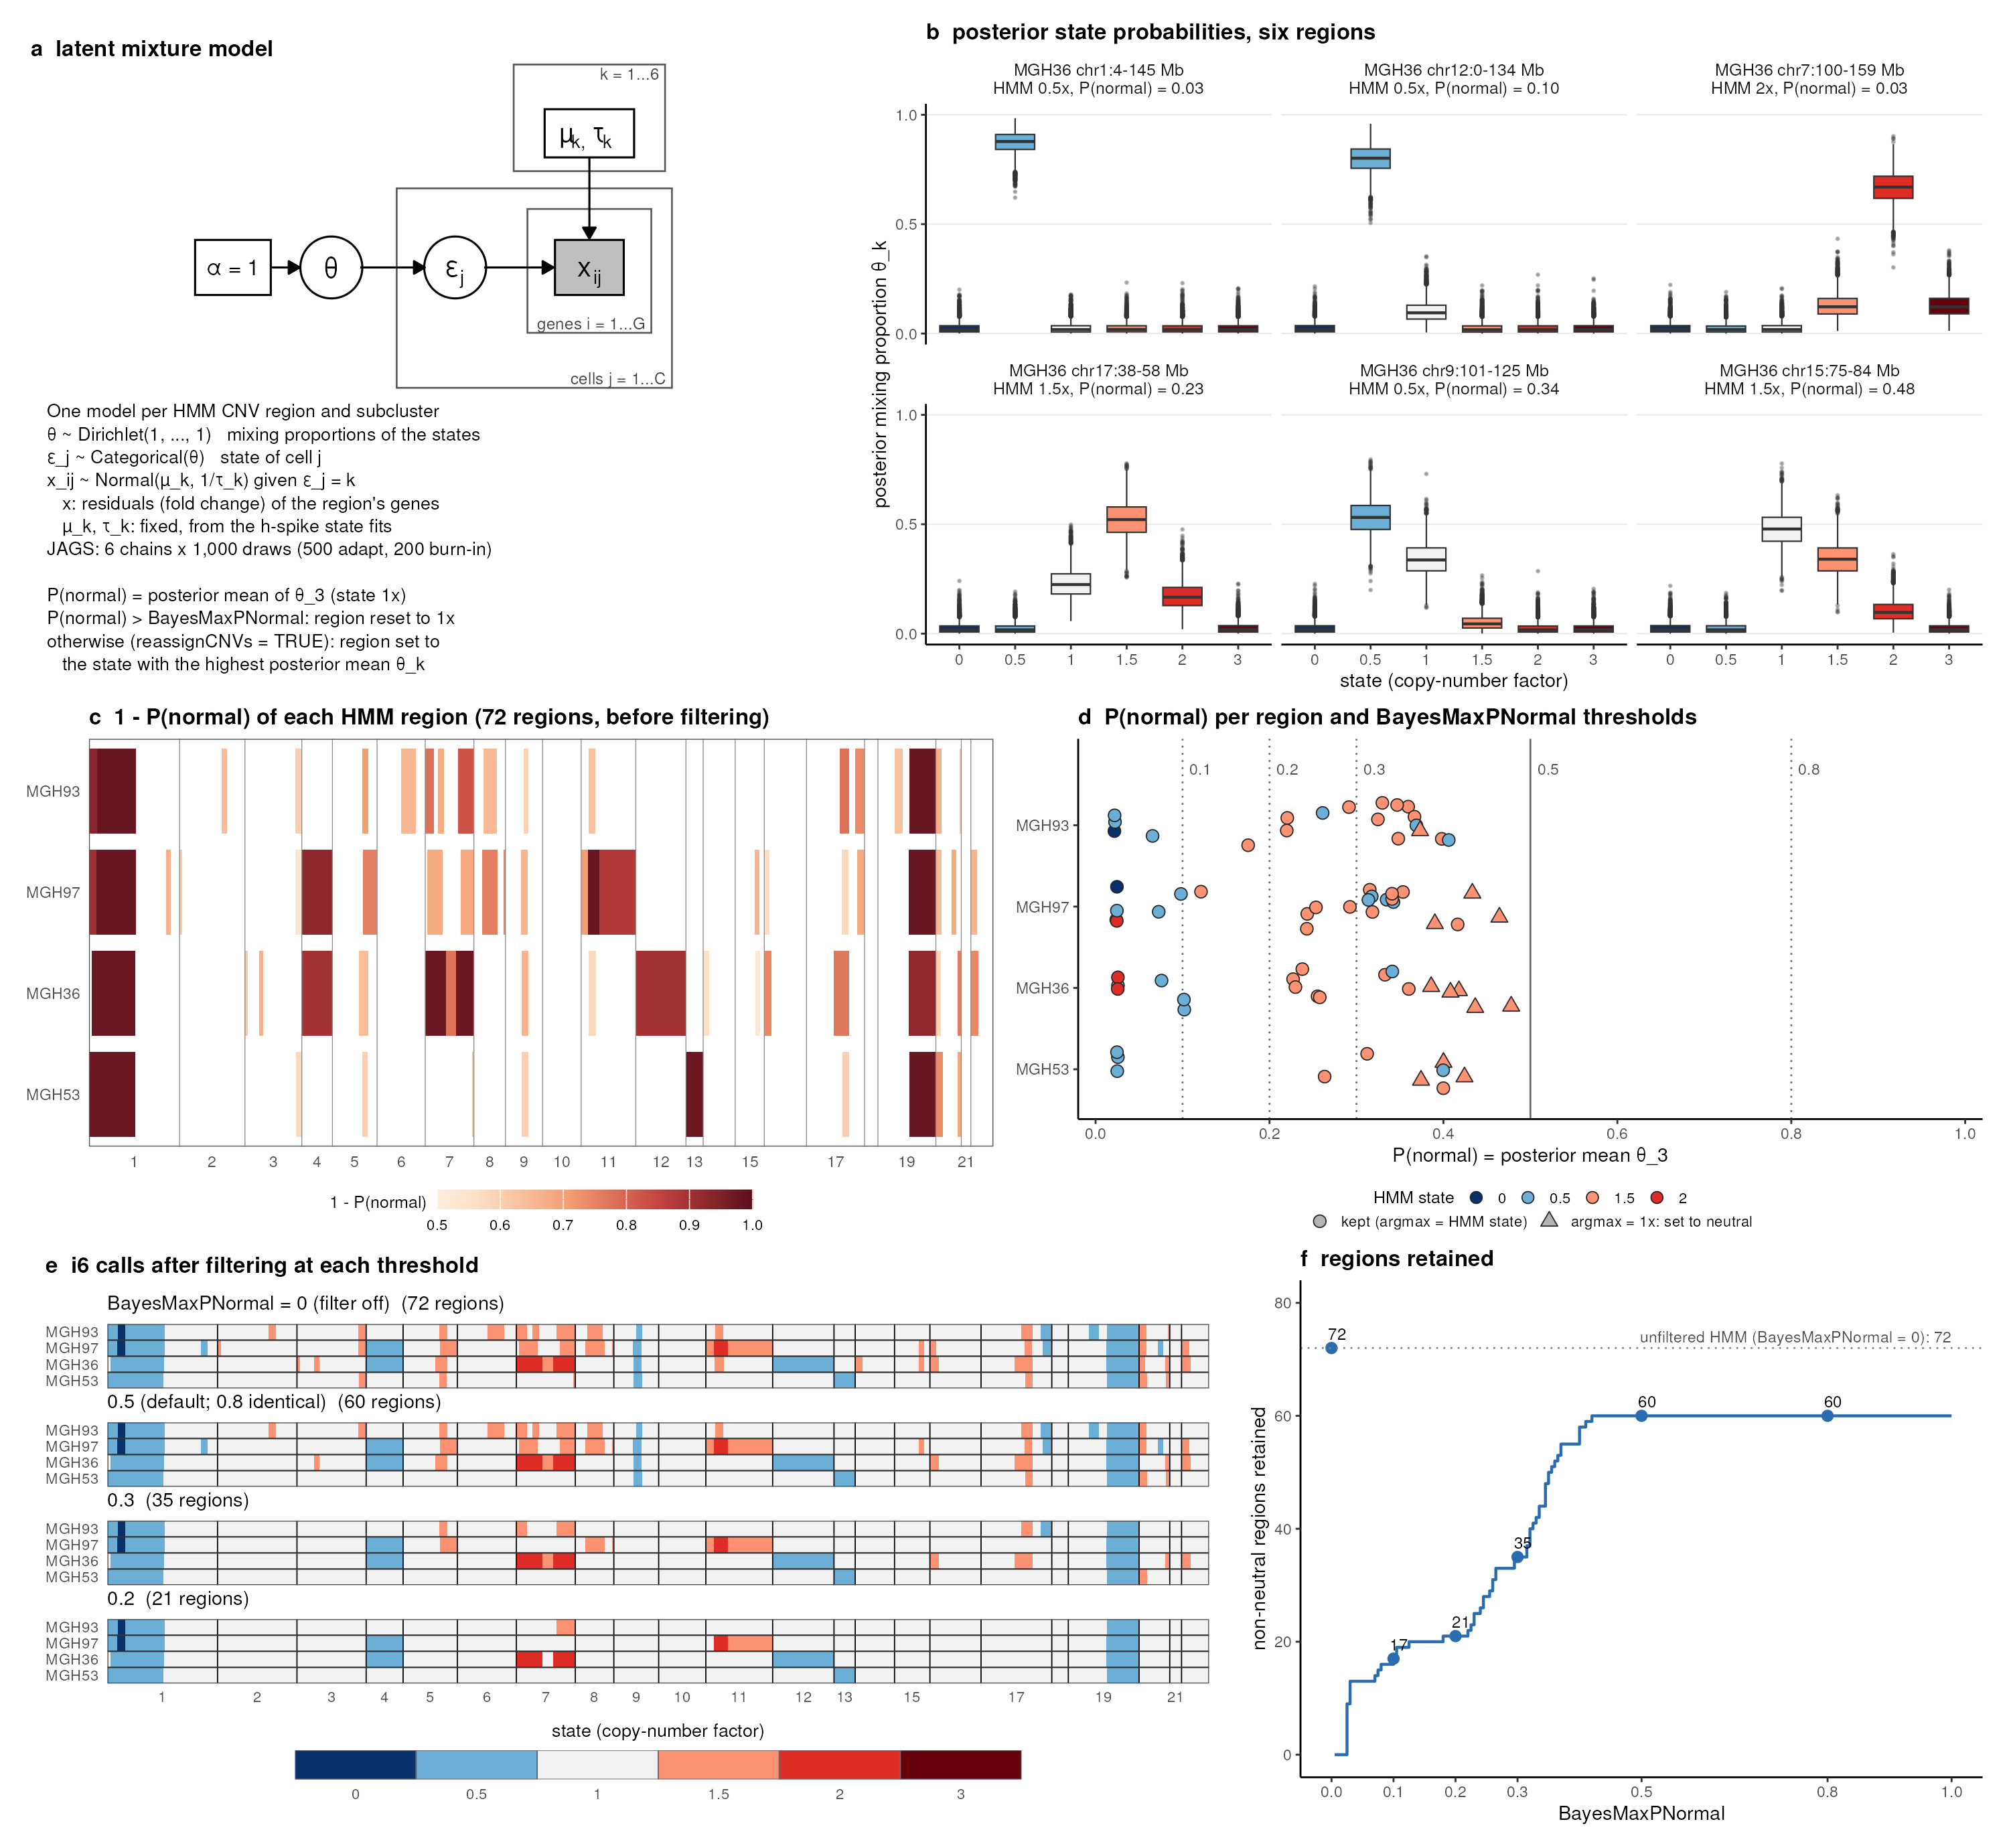
\includegraphics[width=\textwidth]{figures/figS_bayes.png}
\caption{\textbf{Bayesian filtering of HMM calls (extdata oligodendroglioma example).} \textbf{a}, The latent mixture model fitted to each predicted CNV region in each subcluster. The residuals $x_{ij}$ of the region's genes in each cell are normal with the mean $\mu_k$ and precision $\tau_k$ of the cell's state $\varepsilon_j$, fixed at the single-cell values of the h-spike calibration (Supplementary Fig.~\ref{fig:Smodels}d). Cell states are drawn from mixing proportions $\theta$ with a flat Dirichlet prior. P(normal) is the posterior mean of $\theta$ for the neutral state. \textbf{b}, Posterior distributions of $\theta$ (6 chains × 1,000 draws, one chain per state, each started with all cells in that state) for six MGH36 regions, from confident (1p, 1 copy; 7q, 4 copies) to marginal (15q, 3 copies, P(normal) = 0.48). \textbf{c}, 1 $-$ P(normal) for the 72 regions called by the i6 HMM, along the genome (one row per Leiden subcluster, one per tumour). \textbf{d}, P(normal) of each region, coloured by HMM state. Lines mark the BayesMaxPNormal values in \textbf{e--f}. Triangles: regions whose most probable state is neutral, which \texttt{reassignCNVs} resets to neutral (2 copies) even when P(normal) is below the threshold. \textbf{e}, i6 calls after filtering with BayesMaxPNormal = 0 (model off), 0.5 (default; 0.8 gives the same calls), 0.3 and 0.2. \textbf{f}, Number of non-neutral regions retained as a function of BayesMaxPNormal.}
\label{fig:S2}
\end{figure}}

% fig:S3
\expandafter\long\expandafter\def\csname float@fig:S3\endcsname{%
\begin{figure}[p]
\centering
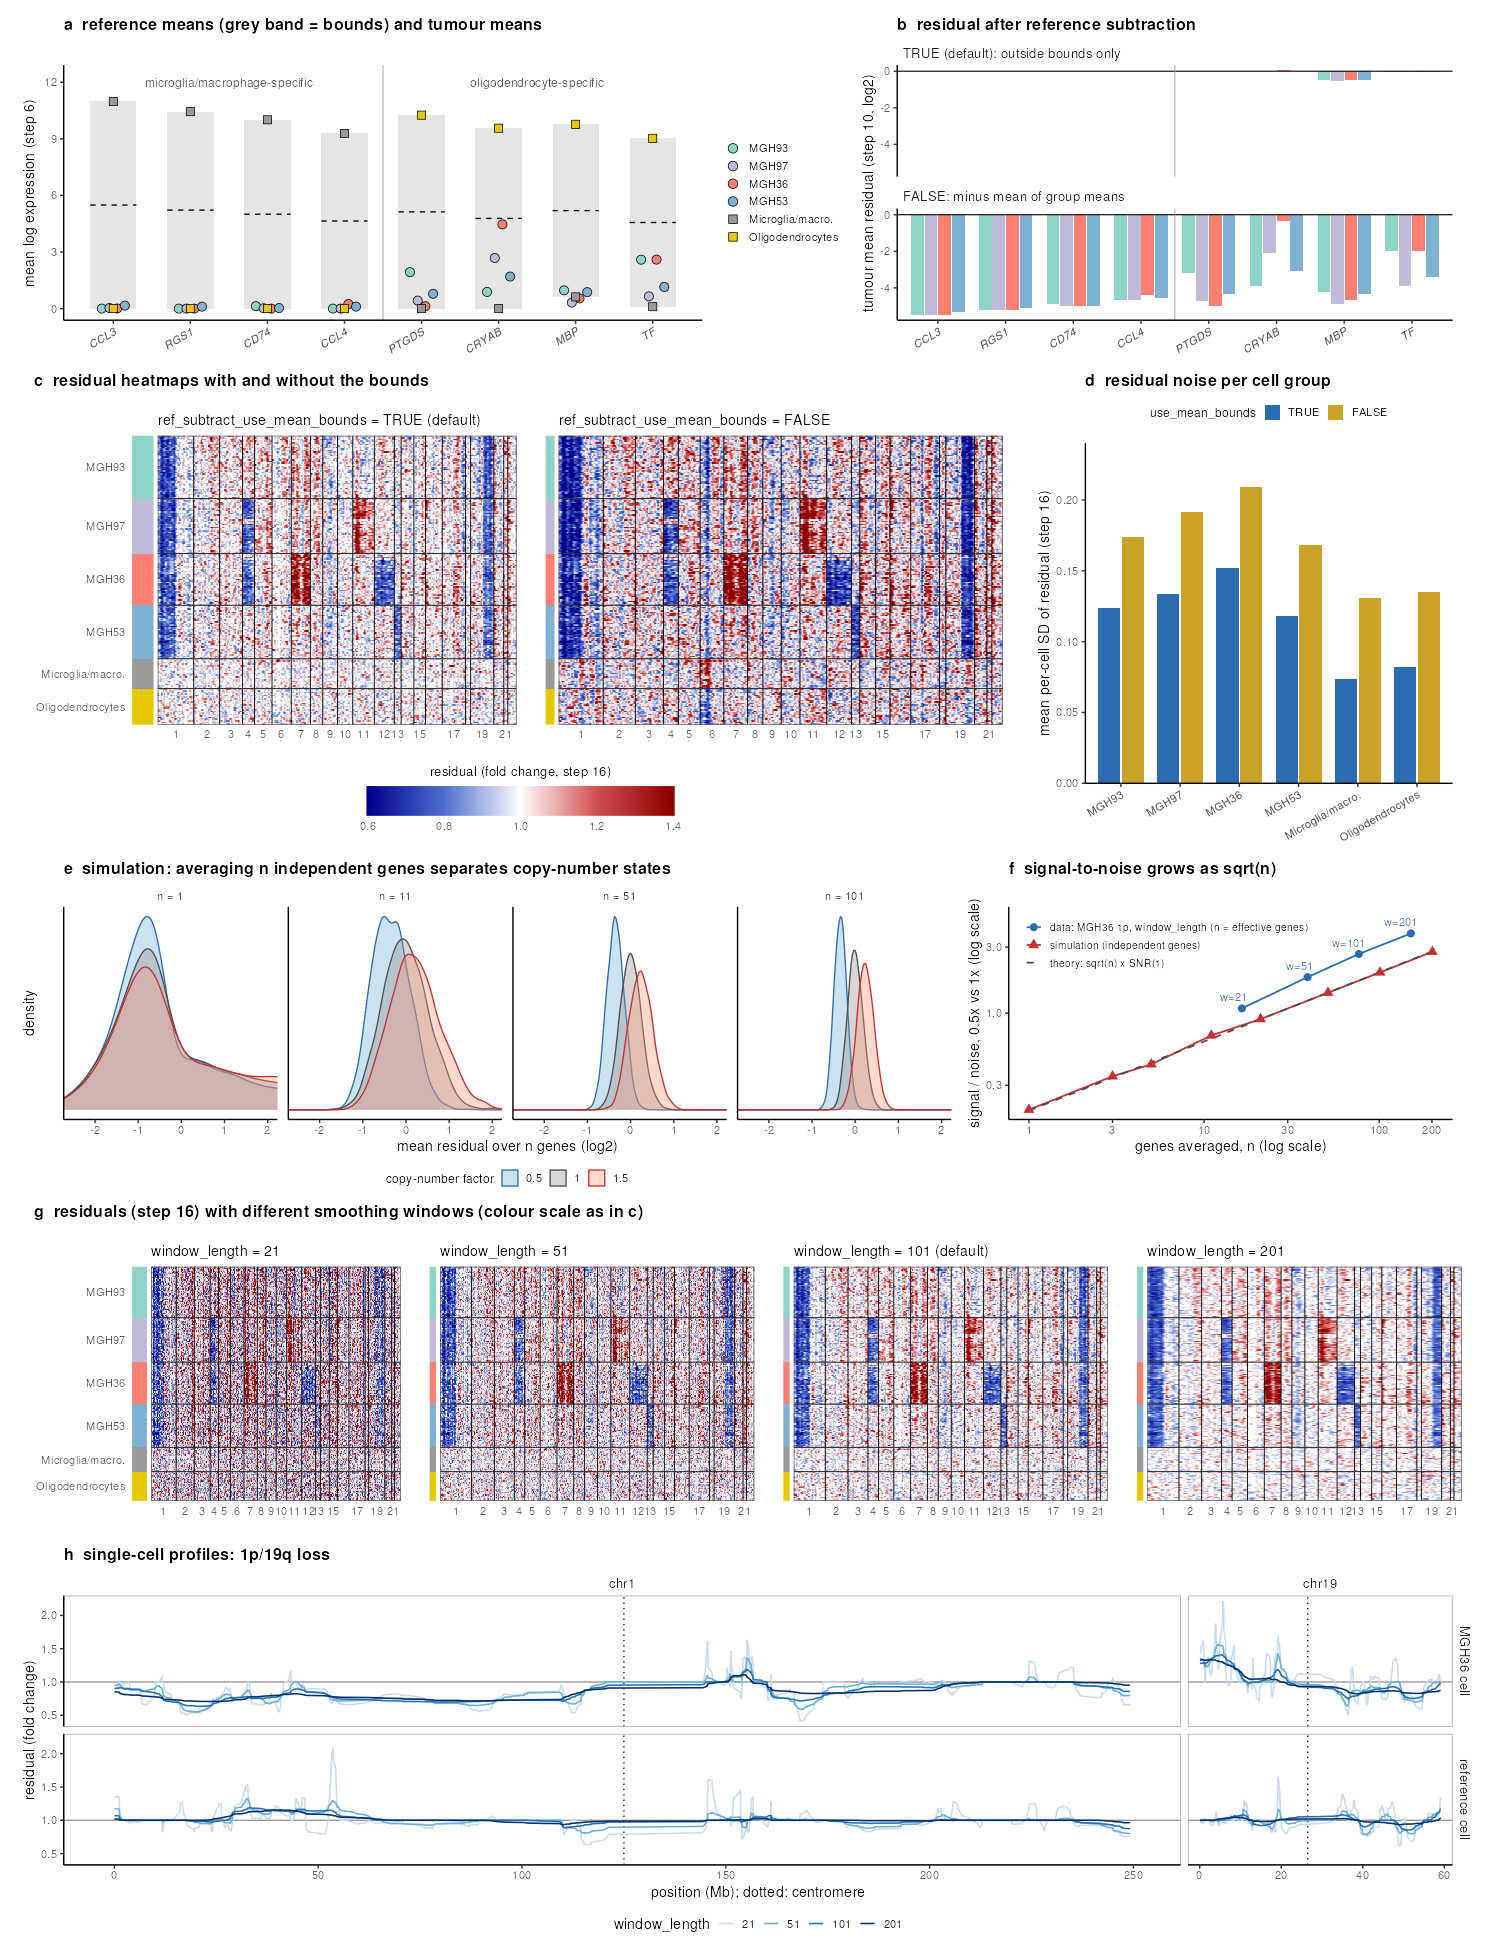
\includegraphics[width=\textwidth]{figures/figS_refsmooth.png}
\caption{\textbf{Reference subtraction with several reference groups, and smoothing.} \textbf{a}, Mean log expression (step 6) of four microglia/macrophage- and four oligodendrocyte-specific genes in the two reference groups (squares) and the four tumours (circles). Grey bands span the reference group means (the bounds); dashed lines show the mean of the group means. \textbf{b}, Mean residual of each tumour after the first reference subtraction (step 10). With \texttt{ref\_subtract\_use\_mean\_bounds = TRUE} (default), values within the bounds are set to 0. Without the bounds, the mean of the group means is subtracted. \textbf{c}, Residuals after smoothing, centring and the second subtraction (step 16) with and without the bounds (same colour scale). \textbf{d}, Mean per-cell SD of the step-16 residuals per cell group. \textbf{e}, Simulation: distributions of the mean residual over n independent genes at copy-number factors 0.5, 1 and 1.5. Counts are negative binomial, with the reference gene means and dispersion of the example data. \textbf{f}, Signal-to-noise (0.5× against 1×) against the number of genes averaged. Shown are the simulation, the $\sqrt{n}$ prediction, and the example data: MGH36 1p loss at \texttt{window\_length} 21, 51, 101 and 201, plotted at the effective number of genes of the triangular kernel (16, 39, 76, 151). \textbf{g}, Step-16 residuals for the four window lengths (colour scale as in c). \textbf{h}, Residuals along chr1 and chr19 of one MGH36 cell and one oligodendrocyte for each window length.}
\label{fig:S3}
\end{figure}}

% fig:S4
\expandafter\long\expandafter\def\csname float@fig:S4\endcsname{%
\begin{figure}[p]
\centering
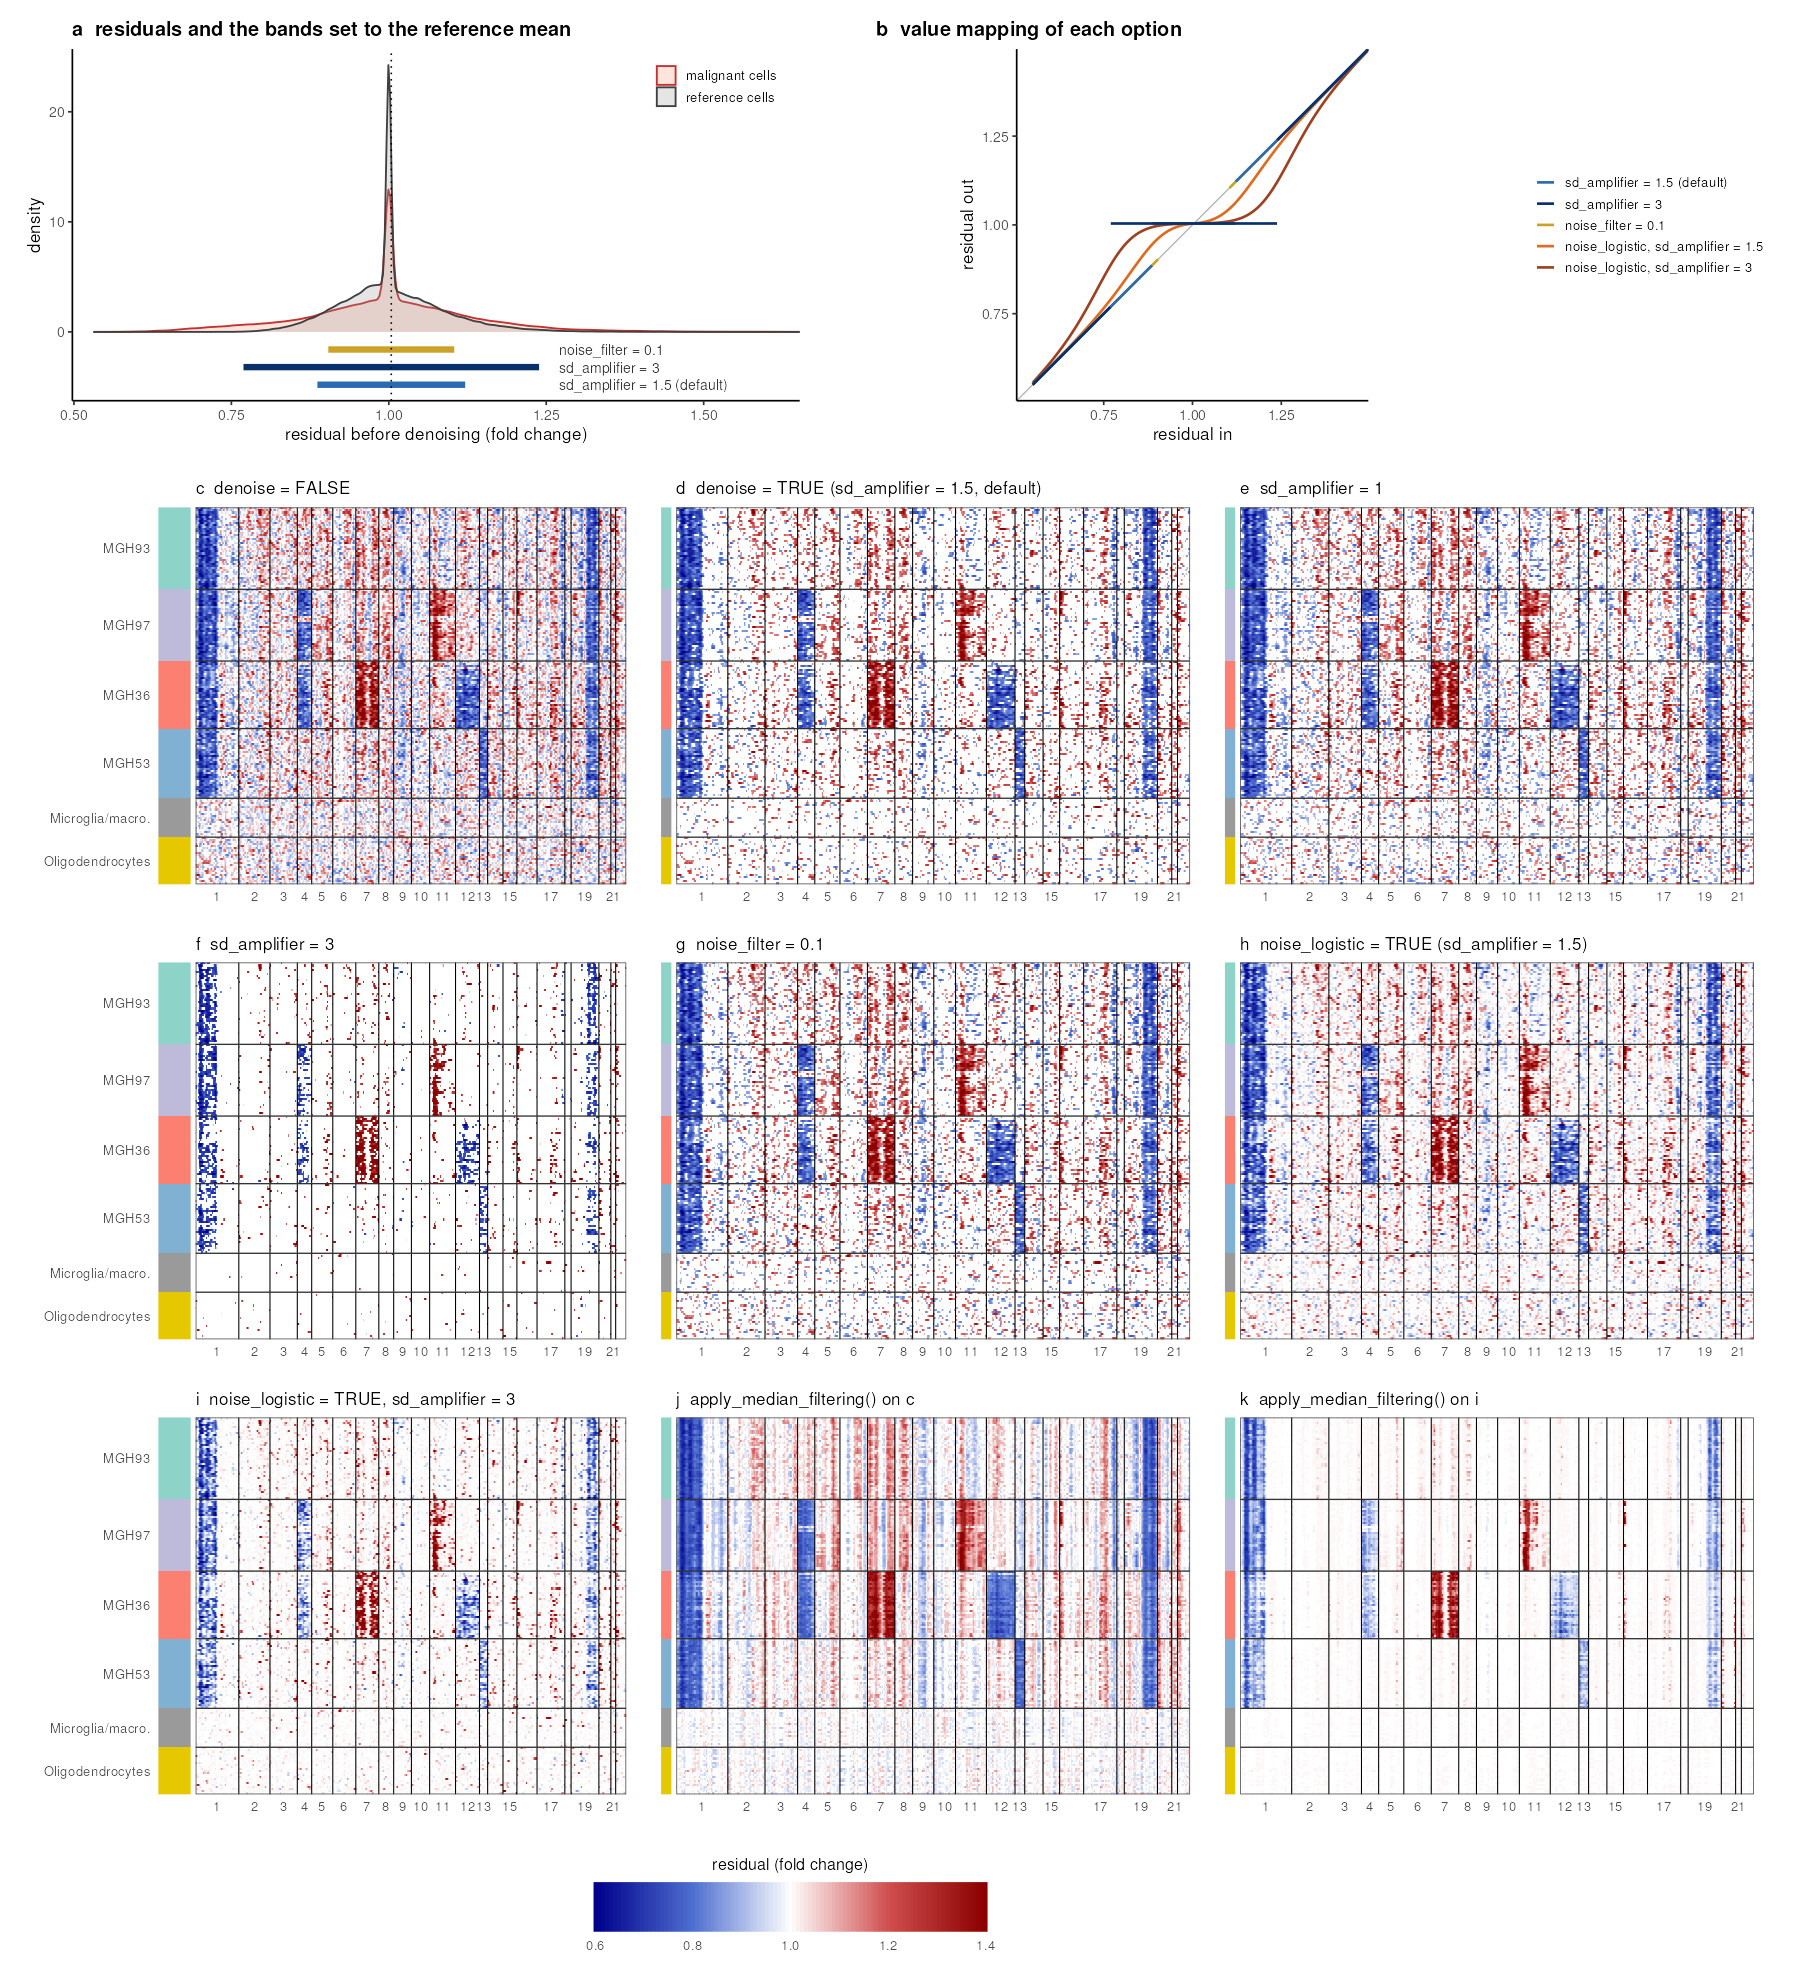
\includegraphics[width=\textwidth]{figures/figS_denoise.png}
\caption{\textbf{Denoising options for the residual heatmap (extdata example).} \textbf{a}, Residuals (fold change, before denoising) of reference and malignant cells. Bars show the ranges set to the reference mean by the default dynamic threshold (reference mean ± 1.5 × the mean per-cell SD of the reference cells, \texttt{sd\_amplifier = 1.5}), by \texttt{sd\_amplifier = 3}, and by a fixed \texttt{noise\_filter = 0.1}. \textbf{b}, Output against input value for each option: the hard thresholds and the logistic shrinkage (\texttt{noise\_logistic = TRUE}, midpoint at the same threshold). \textbf{c--i}, Residual heatmaps without denoising (c), with the default (d), with \texttt{sd\_amplifier} 1 and 3 (e, f), with \texttt{noise\_filter = 0.1} (g), and with logistic shrinkage at \texttt{sd\_amplifier} 1.5 and 3 (h, i). \textbf{j, k}, \texttt{apply\_median\_filtering()} (a separate function, not part of \texttt{run()}; \texttt{window\_size = 7}) applied to c and to i. All panels use the same colour scale. Denoising changes only the displayed residuals; the HMM calls are computed before it and are unaffected.}
\label{fig:S4}
\end{figure}}

% Supplementary Table S2: values from analyses/fig4/metrics_fig4.tsv (this study) and
% analyses/fig4/schmid2025_reported_infercnv_v1.10.tsv (reported by Schmid et al. for v1.10).
\expandafter\long\expandafter\def\csname float@tab:S2\endcsname{%
\begin{table}[p]
\centering
\footnotesize
\caption{\textbf{Agreement with DNA-based copy number.} For each sample and inferCNV score (CNV, mean HMM state after Bayesian filtering; Expr, mean residual expression), the maximal three-class F1 with sensitivity and precision for gains and losses at the optimum, AUC and partial AUC for gains and losses, and the Pearson correlation with the exome truth, over 100-kb bins (Methods). ``v1.10'' rows are the values reported by Schmid et al.~\citep{schmid2025} for inferCNV v1.10 on the same samples; ``this study'' rows are the release code, scored on the bins covered by inferCNV genes (MM199: 1,916 malignant cells, 6,409 bins; BCC06: 1,403 cells, 8,826 bins; BCC06post: 320 cells, 9,509 bins).}
\label{tab:S2}
\setlength{\tabcolsep}{4pt}
\begin{tabular}{@{}llcccccccccc@{}}
\toprule
 & & & \multicolumn{2}{c}{Gain} & \multicolumn{2}{c}{Loss} & \multicolumn{2}{c}{AUC} & \multicolumn{2}{c}{Partial AUC} & \\
\cmidrule(lr){4-5}\cmidrule(lr){6-7}\cmidrule(lr){8-9}\cmidrule(lr){10-11}
Sample & Score & Max.\ F1 & Sens. & Prec. & Sens. & Prec. & Gain & Loss & Gain & Loss & $r$ \\
\midrule
MM199     & CNV, this study  & 0.64 & 0.56 & 0.73 & 0.47 & 0.68 & 0.84 & 0.78 & 0.80 & 0.62 & 0.58 \\
          & CNV, v1.10       & 0.67 & 0.57 & 0.78 & 0.51 & 0.75 & 0.84 & 0.78 & 0.70 & 0.54 & 0.61 \\
          & Expr, this study & 0.64 & 0.69 & 0.65 & 0.45 & 0.70 & 0.83 & 0.79 & 0.79 & 0.66 & 0.51 \\
          & Expr, v1.10      & 0.66 & 0.73 & 0.64 & 0.47 & 0.77 & 0.85 & 0.80 & 0.81 & 0.68 & 0.58 \\
\addlinespace
BCC06     & CNV, this study  & 0.41 & 0.42 & 0.34 & 0.22 & 0.41 & 0.60 & 0.58 & 0.47 & 0.32 & 0.20 \\
          & CNV, v1.10       & 0.42 & 0.35 & 0.36 & 0.26 & 0.41 & 0.60 & 0.59 & 0.32 & 0.24 & 0.21 \\
          & Expr, this study & 0.41 & 0.34 & 0.37 & 0.25 & 0.40 & 0.60 & 0.60 & 0.52 & 0.43 & 0.21 \\
          & Expr, v1.10      & 0.42 & 0.36 & 0.36 & 0.25 & 0.43 & 0.60 & 0.60 & 0.52 & 0.44 & 0.22 \\
\addlinespace
BCC06post & CNV, this study  & 0.41 & 0.33 & 0.48 & 0.24 & 0.33 & 0.62 & 0.58 & 0.49 & 0.22 & 0.23 \\
          & CNV, v1.10       & 0.38 & 0.35 & 0.47 & 0.07 & 0.46 & 0.63 & 0.57 & 0.36 & 0.07 & 0.25 \\
          & Expr, this study & 0.42 & 0.41 & 0.43 & 0.30 & 0.32 & 0.61 & 0.57 & 0.55 & 0.35 & 0.22 \\
          & Expr, v1.10      & 0.43 & 0.47 & 0.43 & 0.33 & 0.32 & 0.64 & 0.58 & 0.58 & 0.37 & 0.25 \\
\bottomrule
\end{tabular}
\end{table}}

% fig:S5
\expandafter\long\expandafter\def\csname float@fig:S5\endcsname{%
\begin{figure}[p]
\centering
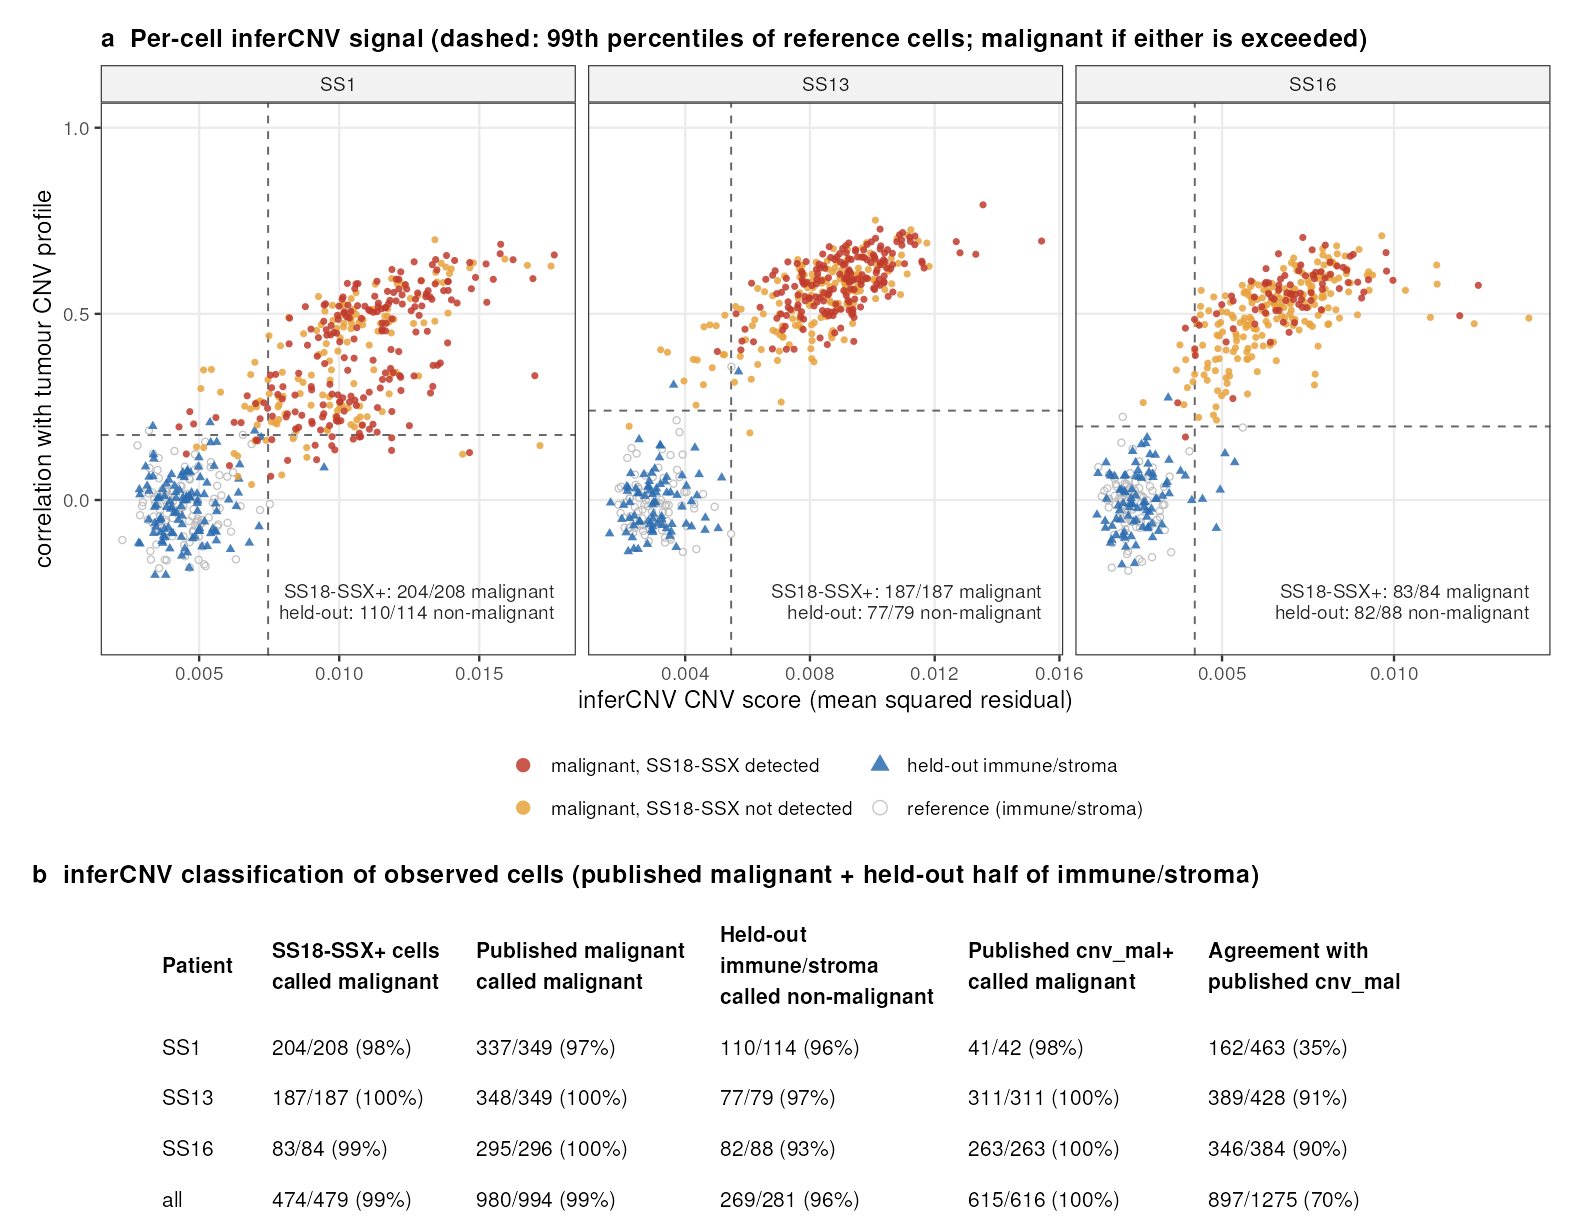
\includegraphics[width=\textwidth]{figures/fig_ss_fusion.png}
\caption{\textbf{inferCNV classification of synovial sarcoma cells compared with SS18--SSX fusion detection.} Smart-seq2 counts, cell annotations and SS18--SSX fusion calls of three synovial sarcomas from the original study \citep{jerbyarnon2021}; inferCNV was run per patient with half of the published immune and stromal cells as the reference (one group per published cluster), and the other half held out and analysed with the published malignant cells. (a) Per-cell CNV score (mean squared residual) against correlation with the tumour's CNV profile, for published malignant cells with and without a detected SS18--SSX transcript (original study), held-out immune and stromal cells, and reference cells. Dashed lines, 99th percentiles of the reference cells; cells beyond either line are classified malignant. (b) Classification per patient, and agreement with the CNV-based labels of the original study.}
\label{fig:S5}
\end{figure}}

% fig:S6
\expandafter\long\expandafter\def\csname float@fig:S6\endcsname{%
\begin{figure}[p]
\centering
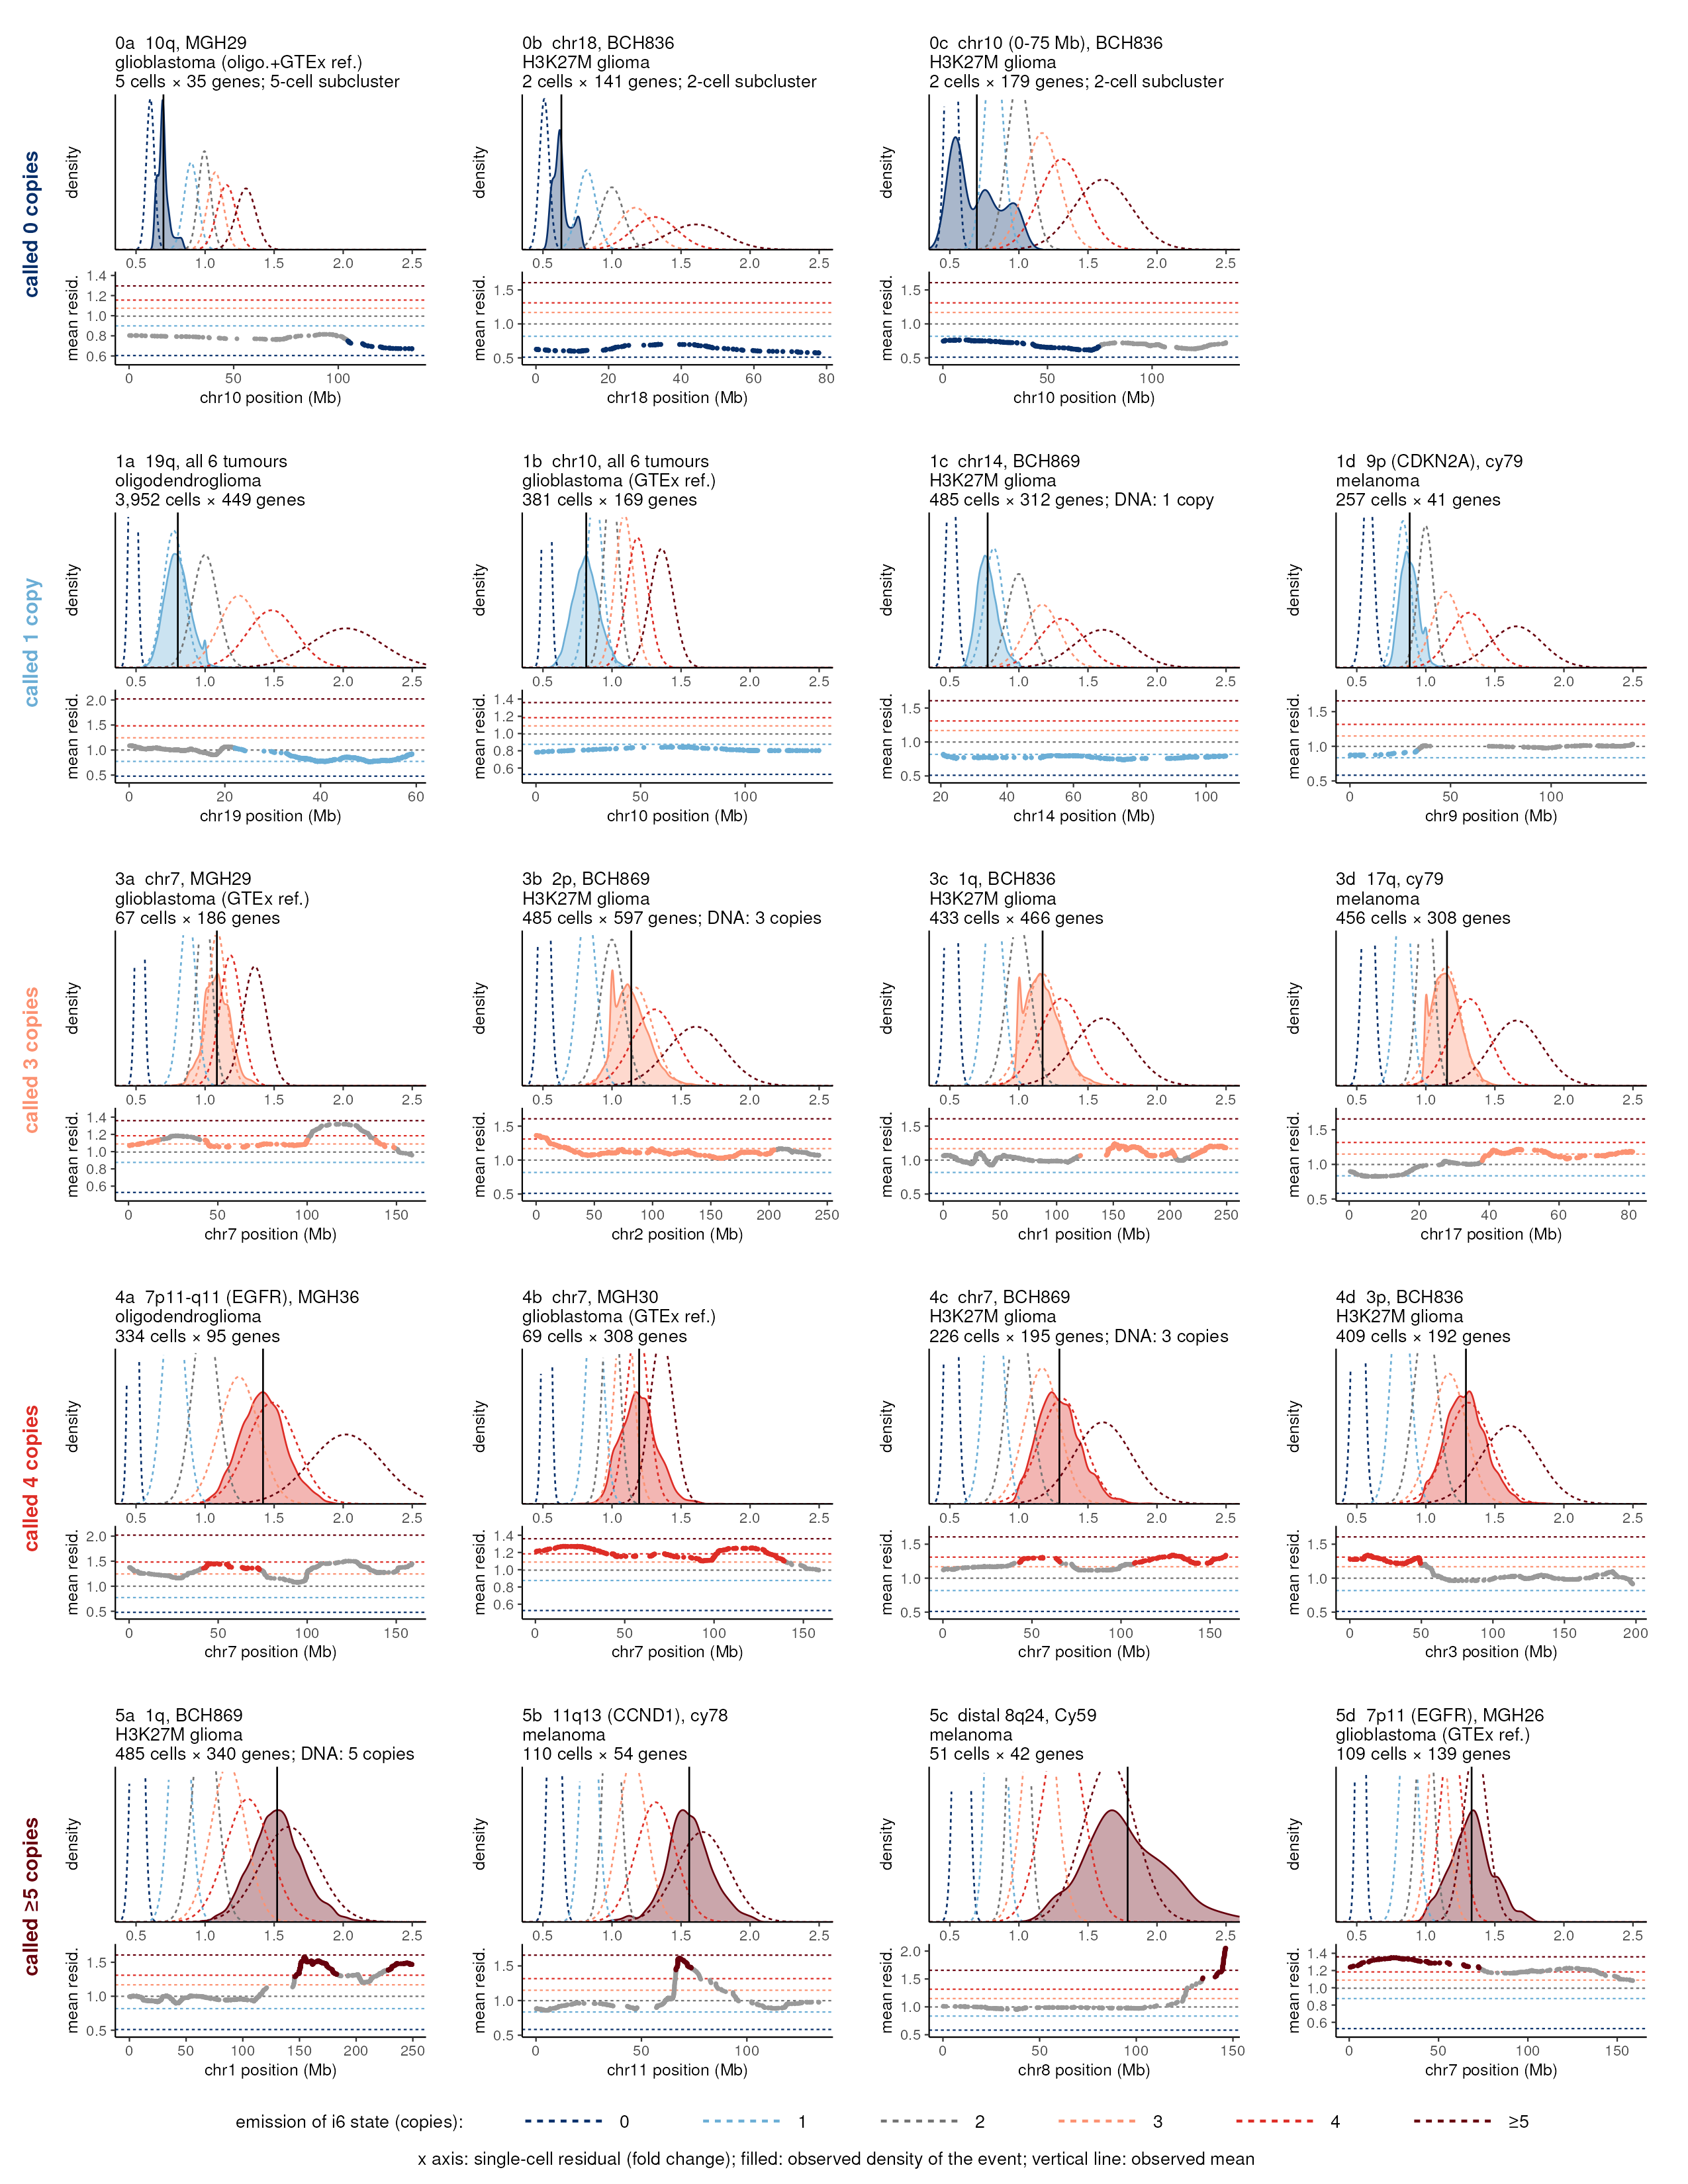
\includegraphics[width=\textwidth]{figures/figS_state_examples.png}
\caption{\textbf{Observed residuals of HMM-called events against the i6 emission densities, by called state.} Events from the Smart-seq2 data sets (oligodendroglioma; glioblastoma with the GTEx or the oligodendrocyte plus GTEx reference; melanoma; H3K27M glioma), grouped by the called i6 state (rows: 0, 1, 3, 4 and $\geq$5 copies). Each event pools the cells and genes of the HMM-called regions of that state (after Bayesian filtering) over the subclusters of a tumour (subclusters of $\geq$10 cells, except in the 0-copy row). Top of each panel, density of the single-cell residuals before denoising (filled; vertical line, mean) against the six emission densities of that run's h-spike (dashed, coloured by state; clipped at the top). Bottom, per-gene mean residual of the same cells along the chromosome (event genes coloured; dashed lines, emission means). DNA, copy number of the BCH869 clones from bulk whole-genome sequencing \citep{filbin2018, huang2024xclone}. For calls of 1 to 4 copies, the residuals centre on the emission of the called state. High-level gains are compressed: the $\geq$5-copy state is open-ended, its emission mean is only 1.36 in the glioblastoma run with scaled data (5d), observed residuals can lie beyond it (5c), and focal amplicons are diluted by smoothing. Uniform gains can be split between adjacent states: 1q of BCH869, 5 copies by DNA, is called as alternating 3-, 4- and $\geq$5-copy segments (only the $\geq$5 segments are shown in 5a), and the 3-copy gain of chromosome 7 is partly called 4 copies (4c). All 0-copy calls come from subclusters of one to five cells, with residuals between the 0- and 1-copy emissions; in subclusters of four or fewer cells the Bayesian filter cannot reset a region to neutral (Supplementary Methods), which is why these calls survive. No homozygous deletion, including of \textit{CDKN2A}, was called. The 10x data sets are not shown because only their denoised residuals were saved.}
\label{fig:S6}
\end{figure}}

% fig:Sres
\expandafter\long\expandafter\def\csname float@fig:Sres\endcsname{%
\begin{figure}[p]
\centering
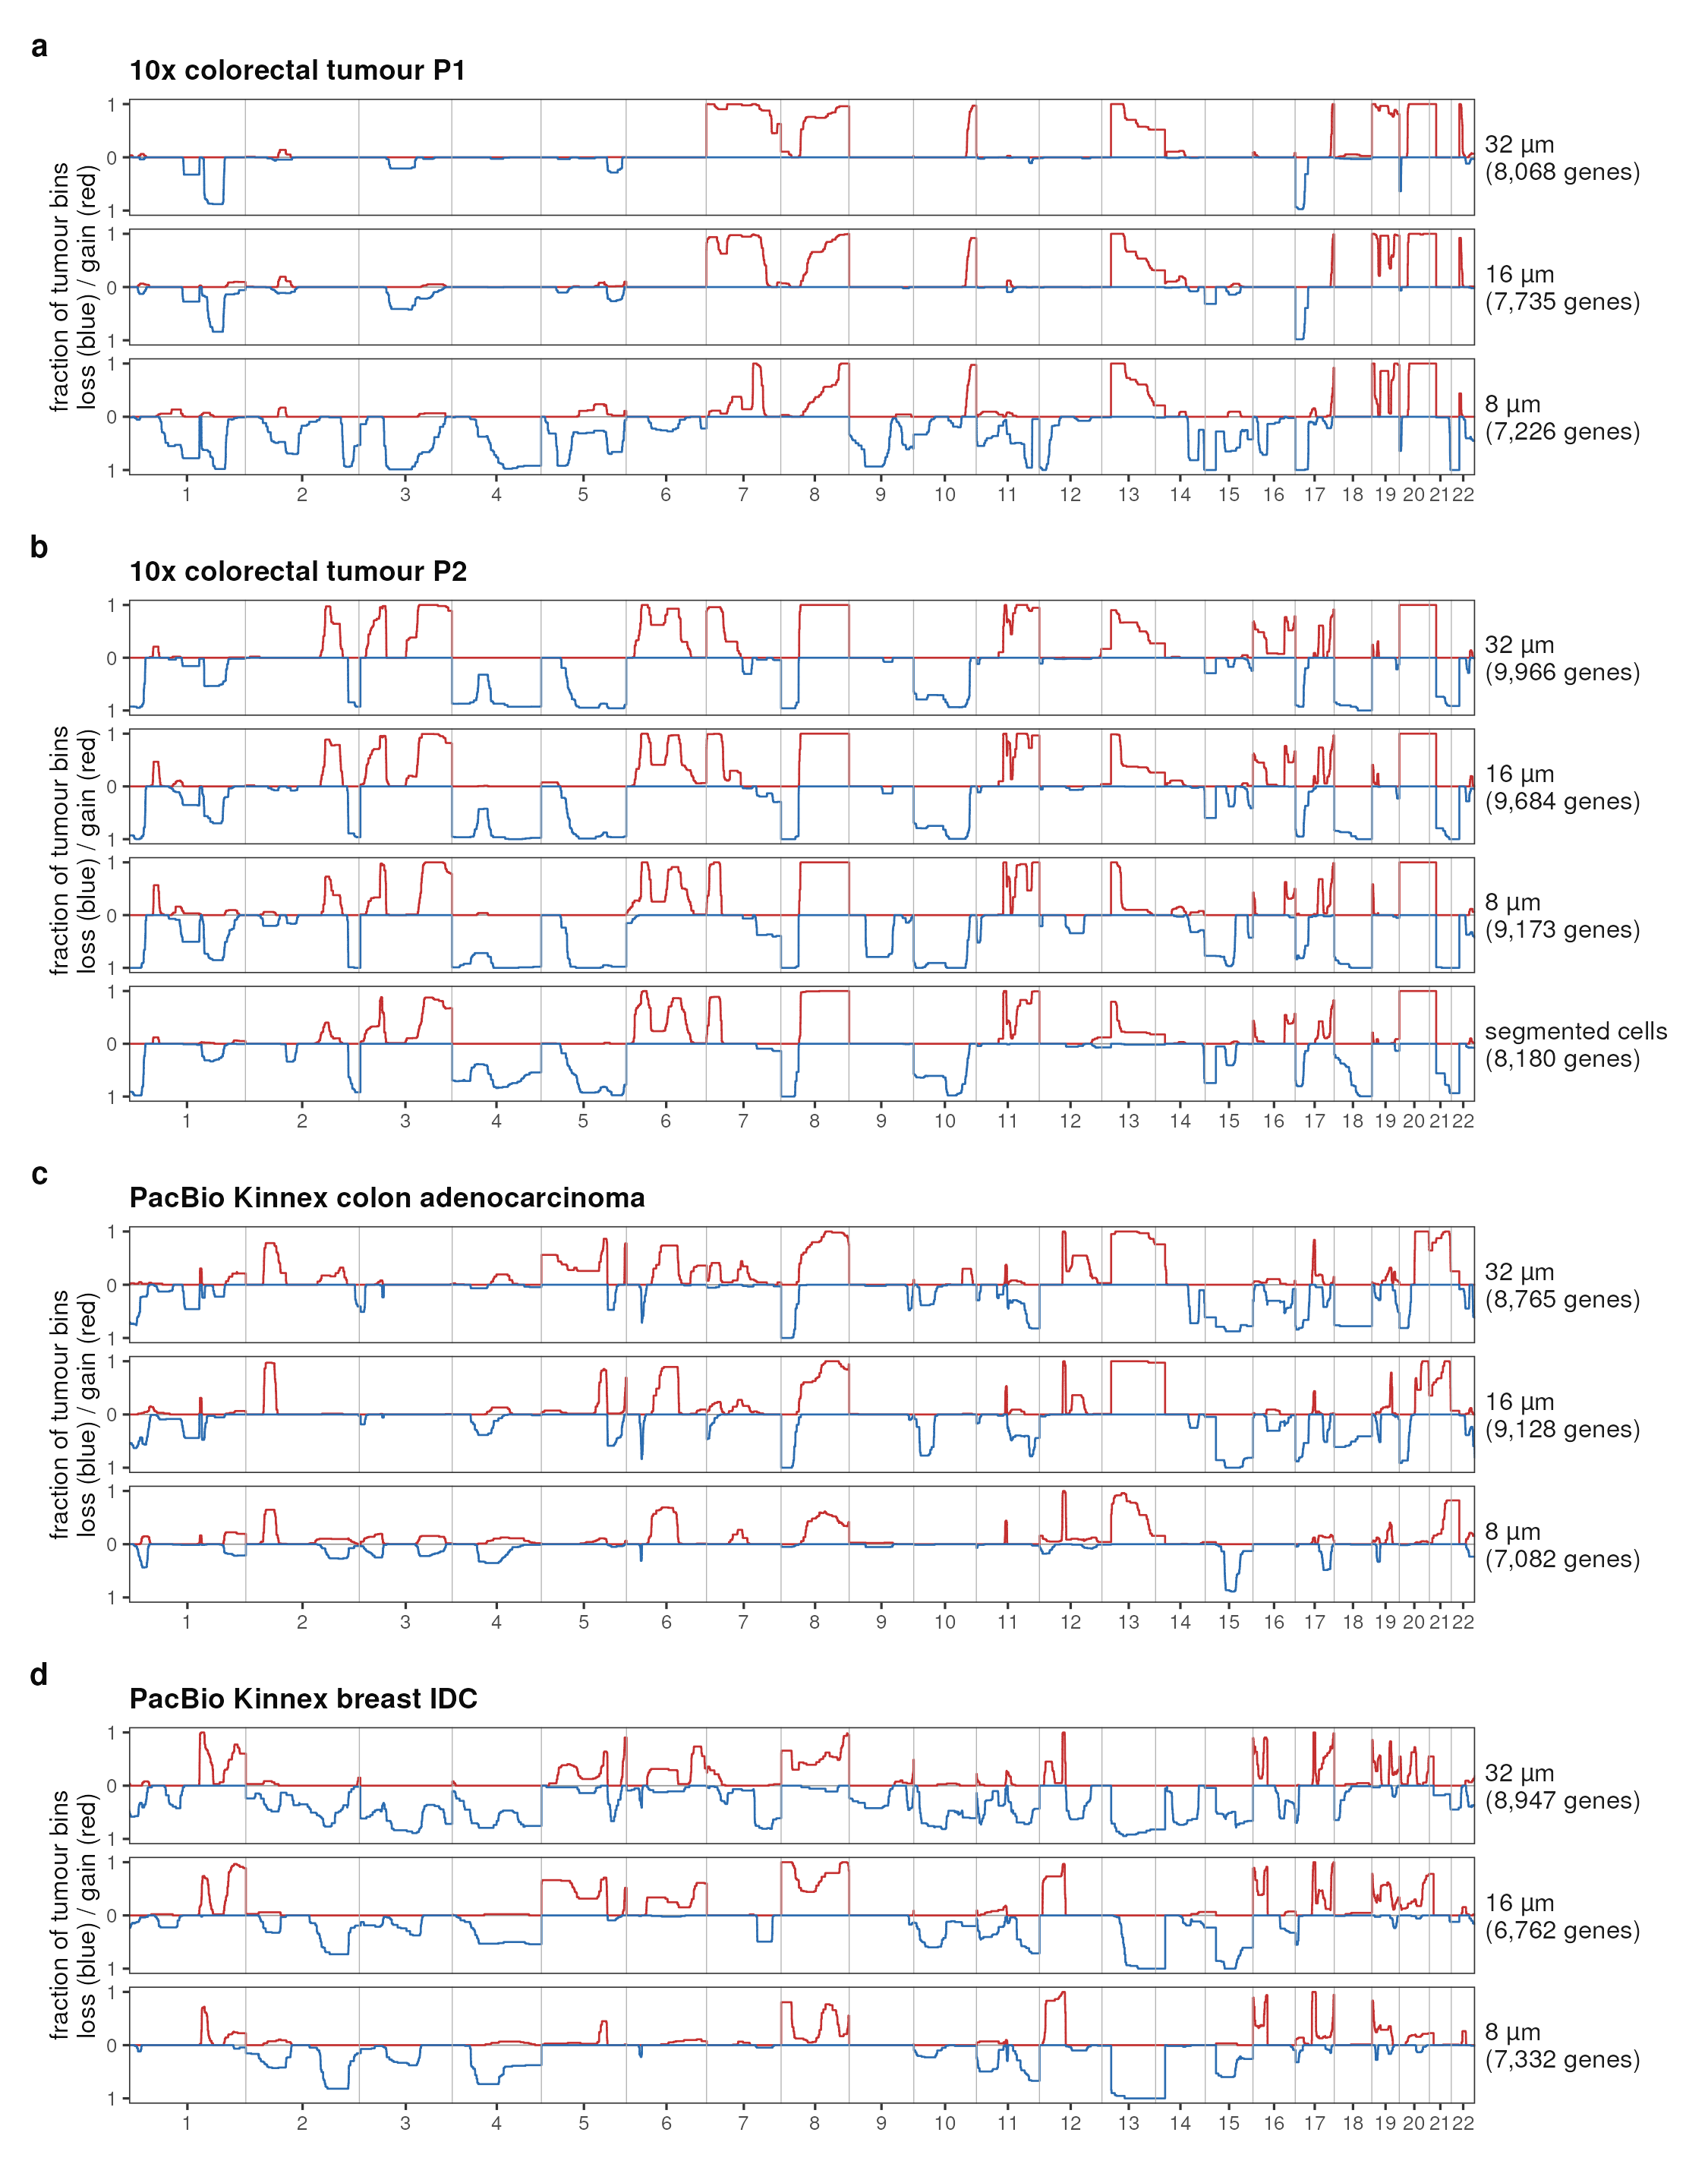
\includegraphics[width=\textwidth]{figures/figS_resolution_profiles.png}
\caption{\textbf{Tumour profiles at three Visium HD bin sizes.} As Fig.~\ref{fig:9}a (\texttt{cutoff\ =\ "auto"}), for the 10x colorectal tumours P1 (a) and P2 (b; with the segmented cells of P2) and the Kinnex colon adenocarcinoma (c) and breast infiltrating ductal carcinoma (d), with bins labelled by marker panels and one reference group per cell type. Fraction of tumour bins called gain (red, up) or loss (blue, down) along chromosomes 1--22, with the number of genes kept.}
\label{fig:Sres}
\end{figure}}
